\documentclass[12pt, a4paper, oneside, openright, titlepage]{book}
\usepackage[utf8]{inputenc}
\raggedbottom
\usepackage{import}


%%%%%%%%%%%%%%%%% Book Formatting Comments:

%%%%%%%%%%%%%%%%%%%%%%%%%%%%%%%%%%%%% for Part

%%%%%%%%%%%%%%%%%%%%%% for chapter

%%%%%%%%%%%%%%%%%%%% for section




%%%%%% PACKAGES %%%%%%%
\usepackage{hyperref}
\hypersetup{
    colorlinks,
    citecolor=black,
    filecolor=black,
    linkcolor=black,
    urlcolor=black
}
\usepackage{amsmath} % Math display options
\usepackage{amssymb} % Math symbols
%\usepackage{amsfonts} % Math fonts
%\usepackage{amsthm}
\usepackage{mathtools} % General math tools
\usepackage{array} % Allows you to write arrays
\usepackage{empheq} % For boxing equations
% \usepackage{mathabx}
% \usepackage{mathrsfs}
\usepackage{nameref}
\usepackage{wrapfig}

\usepackage{soul}
\usepackage[normalem]{ulem}

\usepackage{txfonts}
\usepackage{cancel}
\usepackage[toc, page]{appendix}
\usepackage{titletoc,tocloft}
\setlength{\cftchapindent}{1em}
\setlength{\cftsecindent}{2em}
\setlength{\cftsubsecindent}{3em}
%\setlength{\cftsubsubsecindent}{4em}
\usepackage{titlesec}

%\titleformat{\section}
%  {\normalfont\fontsize{25}{15}\bfseries}{\thesection}%{1em}{}
%\titleformat{\section}
%  {\normalfont\fontsize{20}{15}\bfseries}%{\thesubsection}{1em}{}
%\setcounter{secnumdepth}{1}  
  
  

%\newcommand\numberthis{\refstepcounter{equation}\tag{\theequation}} % For equation labelling
\usepackage[framemethod=tikz]{mdframed}

\usepackage{tikz} % For drawing commutative diagrams
\usetikzlibrary{cd}
\usetikzlibrary{calc}
\tikzset{every picture/.style={line width=0.75pt}} %set default line width to 0.75p

\usepackage{datetime}
\usepackage[margin=1.5in]{geometry}
\setlength{\parskip}{1em}
\usepackage{makeidx}         % allows index generation
\usepackage{graphicx}       % standard LaTeX graphics tool
\usepackage{multicol}        % used for the two-column index
\usepackage[bottom]{footmisc}% places footnotes at page bottom

\usepackage{newtxtext}       % 
\usepackage{newtxmath}       % selects Times Roman as basic font
\usepackage{float}
\usepackage{fancyhdr}
\setlength{\headheight}{15pt} 
\pagestyle{fancy}
\lhead[\leftmark]{}
\rhead[]{\leftmark}

%\usepackage{enumitem}

\usepackage{url}
\allowdisplaybreaks

%%%%%% ENVIRONMENTS %%%
\definecolor{purp}{rgb}{0.29, 0, 0.51}
\definecolor{bloo}{rgb}{0, 0.13, 0.80}



%%\newtheoremstyle{note}% hnamei
%{3pt}% hSpace above
%{3pt}% hSpace belowi
%{}% hBody fonti
%{}% hIndent amounti
%{\itshape}% hTheorem head fonti
%{:}% hPunctuation after theorem headi
%{.5em}% hSpace after theorem headi
%{}% hTheorem head spec (can be left empty, meaning ‘normal’)i





% %%%%%%%%%%%%% THEOREM DEFINITIONS

\spnewtheorem{axiom}{Axiom}[chapter]{\bfseries}{\itshape}


\spnewtheorem{construction}{Construction}[chapter]{\bfseries}{\itshape}

\spnewtheorem{props}{Properties}[chapter]{\bfseries}{\itshape}


\renewcommand{\qedsymbol}{$\blacksquare$}


\numberwithin{equation}{section}

\newenvironment{qest}{
    \begin{center}
        \em
    }
    {
    \end{center}
    }

%%%%%% MACROS %%%%%%%%%
%% New Commands
\newcommand{\ip}[1]{\langle#1\rangle} %%% Inner product
\newcommand{\abs}[1]{\lvert#1\rvert} %%% Modulus
\newcommand\diag{\operatorname{diag}} %%% diag matrix
\newcommand\tr{\mbox{tr}\.} %%% trace
\newcommand\C{\mathbb C} %%% Complex numbers
\newcommand\R{\mathbb R} %%% Real numbers
\newcommand\Z{\mathbb Z} %%% Integers
\newcommand\Q{\mathbb Q} %%% Rationals
\newcommand\N{\mathbb N} %%% Naturals
\newcommand\F{\mathbb F} %%% An arbitrary field
\newcommand\ste{\operatorname{St}} %%% Steinberg Representation
\newcommand\GL{\mathbf{GL}} %%% General Linear group
\newcommand\SL{\mathbf{SL}} %%% Special linear group
\newcommand\gl{\mathfrak{gl}} %%% General linear algebra
\newcommand\G{\mathbf{G}} %%% connected reductive group
\newcommand\g{\mathfrak{g}} %%% Lie algebra of G
\newcommand\Hbf{\mathbf{H}} %%% Theta fixed points of G
\newcommand\X{\mathbf{X}} %%% Symmetric space X
\newcommand{\catname}[1]{\normalfont\textbf{#1}}
\newcommand{\Set}{\catname{Set}} %%% Category set
\newcommand{\Grp}{\catname{Grp}} %%% Category group
\newcommand{\Rmod}{\catname{R-Mod}} %%% Category r-modules
\newcommand{\Mon}{\catname{Mon}} %%% Category monoid
\newcommand{\Ring}{\catname{Ring}} %%% Category ring
\newcommand{\Topp}{\catname{Top}} %%% Category Topological spaces
\newcommand{\Vect}{\catname{Vect}_{k}} %%% category vector spaces'
\newcommand\Hom{\mathbf{Hom}} %%% Arrows

\newcommand{\map}[2]{\begin{array}{c} #1 \\ #2 \end{array}}

\newcommand{\Emph}[1]{\textbf{\ul{\emph{#1}}}}




%% Math operators
\DeclareMathOperator{\ran}{Im} %%% image
\DeclareMathOperator{\aut}{Aut} %%% Automorphisms
\DeclareMathOperator{\spn}{span} %%% span
\DeclareMathOperator{\ann}{Ann} %%% annihilator
\DeclareMathOperator{\rank}{rank} %%% Rank
\DeclareMathOperator{\ch}{char} %%% characteristic
\DeclareMathOperator{\ev}{\bf{ev}} %%% evaluation
\DeclareMathOperator{\sgn}{sign} %%% sign
\DeclareMathOperator{\id}{Id} %%% identity
\DeclareMathOperator{\supp}{Supp} %%% support
\DeclareMathOperator{\inn}{Inn} %%% Inner aut
\DeclareMathOperator{\en}{End} %%% Endomorphisms
\DeclareMathOperator{\sym}{Sym} %%% Group of symmetries


%% Diagram Environments
\iffalse
\begin{center}
    \begin{tikzpicture}[baseline= (a).base]
        \node[scale=1] (a) at (0,0){
          \begin{tikzcd}
           
          \end{tikzcd}
        };
    \end{tikzpicture}
\end{center}
\fi




\newdateformat{monthdayyeardate}{%
    \monthname[\THEMONTH]~\THEDAY, \THEYEAR}
%%%%%%%%%%%%%%%%%%%%%%%

%%% Specific Macros %%%
\usepackage{changepage}
\usepackage{multirow}
\usepackage{pgfplots}

\pgfplotsset{every tick label/.style={inner sep=0pt,font=\scriptsize}}


%%%%%% BEGIN %%%%%%%%%%


\begin{document}

%%%%%% TITLE PAGE %%%%%

\begin{titlepage}
    \centering
    \scshape
    \vspace*{\baselineskip}
    \rule{\textwidth}{1.6pt}\vspace*{-\baselineskip}\vspace*{2pt}
    \rule{\textwidth}{0.4pt}
    
    \vspace{0.75\baselineskip}
    
    {\LARGE Differential Equations: A Complete Guide}
    
    \vspace{0.75\baselineskip}
    
    \rule{\textwidth}{0.4pt}\vspace*{-\baselineskip}\vspace{3.2pt}
    \rule{\textwidth}{1.6pt}
    
    \vspace{2\baselineskip}
    Differential Equations \\
    \vspace*{3\baselineskip}
    \monthdayyeardate\today \\
    \vspace*{5.0\baselineskip}
    
    {\scshape\Large Elijah Thompson, \\ Physics and Math Honors\\}
    
    \vspace{1.0\baselineskip}
    \textit{Solo Pursuit of Learning}
    \vfill
    \enlargethispage{1in}
    \begin{figure}[b!]
    \makebox[\textwidth]{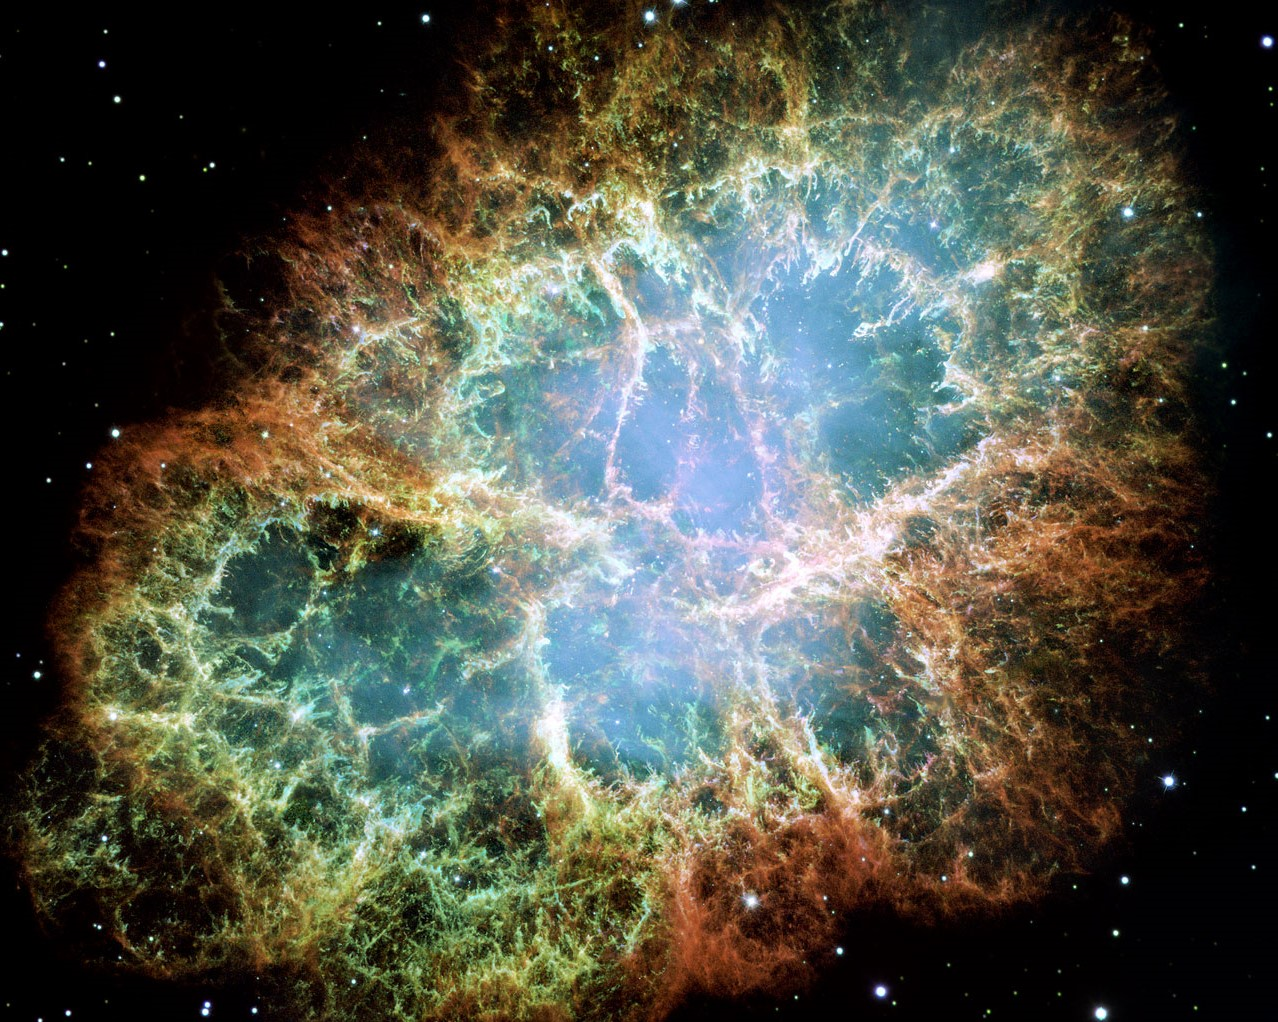
\includegraphics[width=\paperwidth, height =10cm]{../../Crab.jpg}}
    \end{figure}
\end{titlepage}

%%%%%%%%%%%%%%%%%%%%%%%
\tableofcontents








%%%%%%%%%%%%%%%%%%%%%%%%%%%%%%%%%%%%% Part 1. 
\part{Ordinary Differential Equations}

\chapter{Basic Concepts}


\section{Definitions}

\begin{defn}[Differential Equation]
        A \Emph{differential equation} (DE) is an equation connecting an unknown function with some of its derivatives. In general, a DE is of the form \begin{equation}
                F(x,y(x),y'(x),...y^{(n)}(x)) = 0
        \end{equation}
\end{defn}

%{1cm}

\begin{defn}[Order]
        The \Emph{order} of a DE is the order of the highest derivative it contains/
\end{defn}

%{1cm}


\begin{defn}[Dependent and Independent Variables]
        The unknown function in a DE is called the \Emph{dependent variable}, with the variablesw on which it depends being called the \Emph{independent variables}.
\end{defn}


%{1cm}

\begin{defn}[Solution]
        A \Emph{solution} of a DE is a function that satisfies the equation on some open interval $(a,b)$. The graph of a solution to a DE is called a \Emph{solution curve}.
\end{defn}


%{1cm}



\begin{defn}[Graphs]
        A curve $C$ is said to be an \Emph{integral curve} of a DE if every function $y = y(x)$ whose graph is a segment of $C$ is a solution of the DE.
\end{defn}


%{1cm}


\begin{defn}[IVP]
        An \Emph{initial value problem} (IVP) of an nth order DE requires y and its first $n-1$ derivatives to have specified values at some point $x_0$.
\end{defn}


%{1cm}



\begin{defn}[Validity]
        The largest open interval $(a,b)$ that contains $x_0$, on which $y$ is defined and satisfies the DE is the \Emph{interval of validity} of $y$.
\end{defn}



%{1cm}


\begin{defn}[Linear]
        A DE is \Emph{linear} if it is linear with respect to the unknown function and its derivatives.
\end{defn}


%{1cm}


\begin{defn}[Homogeneous]
        A DE is \Emph{homogeneous} if it can be written in the form \begin{equation}
                F(y,y',...,y^{(n)}) = 0
        \end{equation}
        Otherwise, the DE is \Emph{inhomogeneous}.
\end{defn}


%{1cm}


\begin{defn}[Parameter]
        An arbitrary constant in a DE is called a \Emph{parameter} and a solution of a DE with a single parameter edefines a \Emph{one-parameter family of functions}.
\end{defn}




\clearpage 


\chapter{First Order ODEs}



\section{Linear First Order ODEs}

\begin{defn}[Direction Field]
        For a first order DE that can be written in the form \begin{equation}
                y' = f(x,y)
        \end{equation}
        At each point in the $(x,y)$ plane we place an arrow with slope equivalent to the value of $f(x,y)$.
\end{defn}


%{1cm}


\begin{defn}[Linear First Order ODE]
        A \Emph{linear first order ODE} is a DE of the form \begin{equation}
                y'(x) + p(x)y(x) = q(x) \label{eq:1st}
        \end{equation}
\end{defn}


%{1cm}


\begin{defn}[Homogeneous First Order ODE]
        A \Emph{homogeneous linear first order ODE} is a DE of the form \begin{equation}
                y'(x) + p(x)y(x) = 0
        \end{equation}
\end{defn}



%{1cm}


\begin{defn}[First Order Integrating Factor Solution]
        For a linear first order homogeneous differential equation \ref{eq:1st}, we have an \Emph{integrating factor} of the form \begin{equation}
                \mu(x) = e^{\int p(x)dx},\;\frac{d\mu}{dx} = e^{\int p(x)dx}p(x)
        \end{equation}
        We multiply \ref{eq:1st} by this integrating factor and use the product law of differentiation to obtain the solution
        \begin{equation}
                y = e^{-\int p(x) dx}\left[\int q(x)e^{\int p(x)dx}dx + C \right]
        \end{equation}
        Note that the constant of integration for the integrating factor will cancel, so we use the simplest integration constant of 0.
\end{defn}



%{1cm}


\begin{defn}[Autonomous]
        A first order ODE is called \Emph{autonomous} if it does not include the independent variable explicitly \begin{equation}
                y' = f(y)
        \end{equation}
\end{defn}


%{1cm}


\begin{eg}[Logistic Equation]
        The \Emph{logistic equation} is a first order autonomous DE of the form \begin{equation}
                \frac{dN}{dt} = rN\left(1 - \frac{N}{\kappa}\right)
        \end{equation}
        where $\kappa = $ the carrying capacity, and $r = $ the growth rate.
\end{eg}




%{1cm}

\section{Separable Equations}

\begin{defn}[Separable Equations]
        We call a first order DE that can be written in the form \begin{equation}
                \frac{dy}{dx}=f(x)g(y)
        \end{equation}
        \Emph{separable}. To solve we separate functions of $x$ and $y$ and integrate \begin{equation}
                \int\frac{1}{g(y)}dy = \int f(x)dx
        \end{equation}
\end{defn}


%{1cm}


\begin{defn}[Singular Solutions]
        When dividing by $g(y)$ in solving the separable DE above, we lose the \Emph{singular solution} $g(y) \equiv 0$.
\end{defn}


%{1cm}

\section{Bernoulli Equations}

\begin{defn}[Bernoulli Equations]
        Consider a first order DE of the following form: \begin{equation}
                y'(x) + p(x)y(x) = q(x)y^n
        \end{equation}
        If $n = 0$ the DE is linear, if $n = 1$ the DE is linear homogeneous and separable, and if $n \neq 0, 1$ then we have a \Emph{Bernoulli equation}. To solve a Bernoulli equation we divide by $y^{n}$ and substitute $z = y^{1-n}$, so $z' =(1-n)y^{-n}y
        $.
\end{defn}


%{1cm}

\section{Exact Equations}


\begin{defn}[Exact Equation]
        If for the equation \begin{equation}
                M(x,y)dx + N(x,y)dy = 0
        \end{equation}
        we can find a function $F(x,y)$ (called a \Emph{potential function}) so that \begin{equation}
                \frac{\partial F}{\partial x} = M(x,y)\;\text{and}\;\frac{\partial F}{\partial y} = N(x,y)
        \end{equation}
        then we say that the DE is \Emph{exact}, and its general solution is \begin{equation}
                F(x,y) = C
        \end{equation}
\end{defn}


%{1cm}


\begin{defn}[Conditions]
        The equation \begin{equation}
                M(x,y)dx + N(x,y)dy = 0
        \end{equation}
        is exact if and only if \begin{equation}
                \frac{\partial M}{\partial y} = \frac{\partial N}{\partial x},\;\text{or},\;M_y = N_x 
        \end{equation}
\end{defn}


%{1cm}


\begin{thm}[Integrating Factors]
        Let \begin{equation}
                M(x,y)dx + N(x,y)dy = 0
        \end{equation}
        be not exact. Then integrating factors $\mu(x)$, $\mu(y)$, or $\mu(x,y)$ of the form \begin{equation}
                \frac{\mu(x)'}{\mu(x)} = \frac{M_y(x,y) - N_x(x,y)}{N(x,y)}
        \end{equation}
        \begin{equation}
                \frac{\mu(y)'}{\mu(y)} = \frac{N_x(x,y) - M_y(x,y)}{M(x,y)}
        \end{equation}
        and \begin{equation}
                \mu(x,y) = x^ny^m
        \end{equation}
        may make the equation exact.
\end{thm}


%{1cm}


\section{Existence And Uniqueness}


\begin{thm}[Existence]
        Consider the IVP \begin{equation}
                y' = f(x,y),\;y(x_0) =y_0
        \end{equation}
        If there exists an open rectangle \begin{equation}
                R = \{(x,y):a < x < b, c< y < d\}
        \end{equation}
        that contains the point $(x_0,y_0)$, such that $f(x,y)$ is continuous in R, then there is an interval $(a_0,b_0)$ such that a solution of our IVP exists in $(a_0,b_0)$ containing $x_0$.
\end{thm}

%{1cm}



\begin{thm}[Uniqueness]
        If in addition to the conditions of existence we have that $\frac{\partial f}{\partial y}$ is continuous on $R$, the solution is also unique.
\end{thm}


%{1cm}


\begin{rmk}[Linear Equivalent]
        A solution of the IVP for a linear ODE \begin{equation}
                y' + p(x)y = q(x),\;y(x_0)=y_0
        \end{equation}
        has a unique solution on $(a,b)$ containing $x_0$ where $p(x)$ and $q(x)$ are continuous.
\end{rmk}

%{1cm}



\section{Applications}


\begin{defn}[Exponential Growth]
        Exponential growth is characterized by a DE of the form \begin{equation}
                \frac{dN}{dt} = rN
        \end{equation}
        with exponential growth for $r > 0$ and exponential decay for $r < 0$. If $N(0) = N_0$, then $N(t) = N_0e^{rt}$.
\end{defn}


%{1cm}

\begin{defn}[Newton's Law of Cooling]
        Let $T(t) = $ the temperature of an object at time t, and $T_{medium} = $ the temperature of the medium. Then \Emph{Newton's Law of Cooling} states that \begin{equation}
                \frac{dT}{dt} = k(T_{medium}-T(t))
        \end{equation}
        This equation is separable and linear, and gives us a general solution of the form: \begin{equation}
                T(t) = T_{medium} + (T_0 - T_{medium})e^{-kt}
        \end{equation}
        where $T(0) = T_0$
\end{defn}


%{1cm}


\begin{defn}[Mixing Problems]
        Let $V(t) = $ the volume of liquid at time t, $Q(t) = $ the amount of substance desolved in the solution, $c_{in} = $ the inflow of concentration, $c_{out} = $ the outflow concentration, $r_{in} = $ the inflow rate, and $r_{out} = $ is the outflow rate. If well mixed, $c_{out} = \frac{Q(t)}{V(t)}$. Let $V(0) = V_0$, so we have the equation \begin{equation}
                V(t) = V_0 + (r_{in} - r_{out})t
        \end{equation}
        and we obtain the differential equation \begin{equation}
                \frac{dQ}{dt} = c_{in}r_{in} -c_{out}r_{out} = c_{in}r_{in} - \frac{Q(t)r_{in}}{V_0+(r_{in}-r_{out})t} 
        \end{equation}
\end{defn}

%{1cm}








\clearpage

\chapter{Second Order Linear ODEs}

\section{Constant Coefficients}

\begin{defn}[Characteristic Equation]
        Given the following linear second order homogeneous DE with constant coefficients \begin{equation}
                y'' + by' + cy = 0 
        \end{equation}
        we have the \Emph{characteristic equation} \begin{equation}
                \lambda^2 + b\lambda + c = 0
        \end{equation}
        This equation results from looking for a solution in the form $y = e^{\lambda x}$.
\end{defn}



%{1cm}

\bgroup
\def\arraystretch{1.5}
\begin{table}[H]
        \centering
        \caption{Solutions for the linear homogeneous DE with constant coefficients, $y'' + by' + c = 0$.}
        \begin{tabular}{c|c}
                Roots of the & General \\ 
                Characteristic Equation & Solution \\ \hline
                $\lambda_1 \neq \lambda_2$ (real) & $C_1e^{\lambda_1 x}+C_2e^{\lambda_2 x}$ \\
                $\lambda_1 = \lambda_2 = \lambda$ (real) & $(C_1+C_2x)e^{\lambda x}$ \\
                $\lambda_{1,2} = \alpha \pm \beta i$ (complex) & $e^{\alpha x}[C_1cos(\beta x) + C_2sin(\beta x)]$ \\
        \end{tabular}
\end{table}
\egroup



%{1cm}


\section{General Theory}

Consider the linear second order ODE \begin{equation}
        y''(x)+b(x)y'(x)+c(x)y=f(x)
\end{equation}


\begin{thm}[Existence and Uniqueness]
         If $b(x)$, $c(x)$, and $f(x)$ are continuous in the above ODE, in an open interval $I$, containing $x_0$, then the solution of this ODE with an initial condition $y(x_0) = y_0$ exists and is unique on the open interval $I$ for any $y_0$.
\end{thm}

%{1cm}


\begin{thm}[Superposition Principle]
        If $y_1$ and $y_2$ are solutions of the complementary homogeneous ODE to our above ODE, then for any $C_1$ and $C_2$, the \Emph{linear combination} $y = C_1y_1+C_2y_2$ is also a solution.
\end{thm}


%{1cm}


\begin{defn}[Wronskian]
        The value \begin{equation}
                W[y_1\;y_2](x) = \begin{vmatrix}y_1(x) & y_2(x) \\
                y'_1(x) & y'_2(x) \end{vmatrix} = y_1(x)y'_2(x) - y_2(x)y'_1(x) 
        \end{equation}
        is called the \Emph{Wronskian} of the functions $y_1$ and $y_2$. Two functions $y_1$ and $y_2$ are \Emph{linearly independent on I} if the identity $C_1y_1(x) + C_2y_2(x) = 0$ on $I$ (for any $x \in I$) is satisfied for only $C_1 = C_2 = 0$. If $W[y_1\;y_2](x)\neq 0$ for all $x \in I$, then $y_1$ and $y_2$ are linearly independent.
\end{defn}

%{1cm}


\begin{thm}[Abel's Formula]
        If $y_1$ and $y_2$ are solutions of our complementary homogeneous equation, then their Wronskian is \begin{equation}
                W(x) = W(x_0)e^{-\int\limits_{x_0}^xb(t)dt}
        \end{equation}
        where $x_0$ is the value for our initial condition.
\end{thm}




%{1cm}

\begin{thm}[The General Solution (Homogeneous)]
        If $y_1$ and $y_2$ are two solutions of our homogeneous complementary equation such that $W[y_1\;y_2](x)\neq 0$ at some $x$, then the general solution of the homogeneous DE is a linear combination $y(x) = C_1y_1(x) + C_2y_2(x)$.
\end{thm}


%{1cm}


\begin{thm}[The General Solution (Inhomogeneous)]
        A general solution of our ODE is a sum of the general solution of the complementary homogeneous equation and a particular solution \begin{equation}
                y_{gen} = y_{part} + y_{hom}
        \end{equation}
\end{thm}

%{1cm}


\section{Method of Undetermined Coefficients}


\bgroup
\def\arraystretch{1.5}
\begin{table}[H]
        \centering
        \caption{Particular solutions of the second order linear ODE $y''(x)+b(x)y'(x)+c(x)y=f(x)$.}
        \begin{tabular}{c|c|c}
                Right Hand & $\lambda$ is a root of & Particular \\
                Side & multiplicity m & Solution \\ \hline
                $P_n(x)$ & $\lambda = 0$ & $x^mQ_n(x)$ \\
                $e^{kx}P_n(x)$ & $\lambda = k$ & $x^me^{kx}Q_n(x)$ \\
                $e^{kx}\cos(\beta x)P_n(x)$ or $e^{kx}\sin(\beta x)P_n(x)$ & $\lambda = k \pm \beta i$ & $x^me^{kx}[Q_n(x)\cos(\beta x) + R_n(x)\sin(\beta x)]$ \\
        \end{tabular}
\end{table}
\egroup


%{1cm}

\begin{eg}[Resonance]
        We say that an ODE of the form \begin{equation}
                y'' + \omega^2y = 0
        \end{equation}
        is a \Emph{harmonic oscillator}. Suppose we have an inhomogeneous equation $$y''+9y=-18\cos(3t)$$ with a solution $$-3t\sin(t)$$ Observe that the external driving force is bound, but our solution is unbounded: this is an example of the phenomenon of \Emph{resonance}.
\end{eg}

%{1cm}


\section{Variation of Parameters}


\begin{defn}[Variation of Parameters]
        The method of \Emph{Variation of Parameters} aims to find a particular solution to ODEs of the form \begin{equation}
                y''(x) + p(x)y'(x) + q(x)y(x) = f(x)
        \end{equation} 
        of the form \begin{equation}
                y_{part} = C_1(x)y_1(x) + C_2(x)y_2(x)
        \end{equation}
        where $C_1(x)$ and $C_2(x)$ are unknown function to be determined, and $y_1(x)$ and $y_2(x)$ are solutions of the complementary homogeneous DE. In our solution we assume $C_1'y_1 + C_2'y_2 = 0$. Our end result is a system of the form \begin{equation}
                \begin{matrix} C_1'y_1 + C_2'y_2 =0 \\ C_1'y_1' + C_2'y_2' = f(x) \end{matrix}
        \end{equation}
        Solving the system or using Cramer's rule gives solutions for the unknown functions of \begin{equation}
                C_1 = -\int\frac{y_2f}{W[y_1\;y_2]}dx,\;C_2 = \int\frac{y_1f}{W[y_1\;y_2]}dx
        \end{equation}
\end{defn}




%\clearpage

\chapter{Higher Order Linear ODEs}


\section{General Theory}

\begin{defn}[n-th Order Linear ODE]
        We consider an n-th order linear ODE \begin{equation}
                L[y]=y^{(n)}+a_{n-1}(x)y^{(n-1)}+\hdots +a_1(x)y'+a_0(x)y =f(x)
        \end{equation}
        with a corresponding homogeneous equation \begin{equation}
                L[y] = 0
        \end{equation}
        For both ODEs we can describe the initial conditions as \begin{equation}
                y(x_0) = y_0,\;y'(x_0) = y_0',...,y^{(n-1)}(x_0)=y_0^{(n-1)}
        \end{equation}
\end{defn}


%{1cm}


\begin{thm}[Existence and Uniqueness]
        If the functions $a_{n-1},...,a_1,a_0,f$ are continuous in an open interval $(\alpha,\beta)$ containing $x_0$, then the IVP has a unique solution on $(\alpha,\beta)$.
\end{thm}


%{1cm}


\begin{thm}[Superposition Principle]
        If $y_1,y_2,...,y_k$ are solutions of the homogeneous ODE $L[y] = 0$, then for any constants $C_1,C_2,...,C_k$, a linear combination \begin{equation}
                y = C_1y_1+C_2y_2+\hdots + C_ky_k
        \end{equation}
        is also a solution. The solutions $y_1,y_2,...,y_k$ are \Emph{linearly independent} on $(\alpha,\beta)$ if $$C_1y_1(x)+\hdots+C_ky_k(x) = 0$$ for any $x \in (\alpha,\beta)$ only for $C_1=...=C_k=0$.
\end{thm}


%{1cm}


\begin{defn}[Fundamental Set]
        If solutions $y_1,...,y_n$ are linearly independent, they form a \Emph{fundamental set} $\{y_1,...,y_n\}$.
\end{defn}


%{1cm}


\begin{thm}[General Solution]
        If $\{y_1,...,y_n\}$ is a fundamental set (linearly independent) set of solutions of $L[y] = 0$, then the general solution is \begin{equation}
                y = C_1y_1 + \hdots + C_ny_n
        \end{equation}
        Solutions are linearly independent if the Wronskian \begin{equation}
                W[y_1,y_2,...,y_n](x) = \begin{vmatrix} y_1 & y_2 & \hdots & y_n \\ y_1' & y_2' & \hdots & y_n' \\ \hdots & \hdots & \hdots & \hdots \\ y_1^{(n-1)} & y_2^{(n-1)} & \hdots & y_n^{(n-1)} \end{vmatrix} \neq 0
        \end{equation}
        for some $x$ in the interval where we consider our homogeneous DE.
\end{thm}



%{1cm}


\begin{thm}[Abel's Theorem]
        The Wronskian of our linear homogeneous DE can be represented by \begin{equation}
                W(x) = W(x_0)e^{-\int\limits_{x_0}^xa_{n-1}(x)dx}
        \end{equation}
        Thus, W is either identically equal to zero or does not vanish.
\end{thm}


%{1cm}


\begin{thm}[Inhomogeneous General Solution]
        If $y_{part}$ is a solution of our inhomogeneous linear DE and $y_{hom}$ is the general solution of the homogeneous linear DE, then the general solution of our inhomogeneous linear DE is \begin{equation}
                y = y_{hom} + y_{part}
        \end{equation}
\end{thm}


%{1cm}


\section{Constant Coefficients}


\begin{defn}[Constant Coefficients]
        In this section we consider the linear homogeneous DE with constant coefficients \begin{equation}
                y^{(n)}+a_{n-1}y^{(n-1)}+\hdots+a_1y'+a_0y = 0
        \end{equation}
        and the linear inhomogeneous DE with constant coefficients \begin{equation}
                y^{(n)}+a_{n-1}y^{(n-1)}+\hdots+a_1y'+a_0y = f(t)
        \end{equation}
\end{defn}


%{1cm}


\begin{defn}[Characteristic Equation]
        For the homogeneous linear DE with constant coefficients, we look for solutions of the form $y = e^{\lambda x}$, which gives the \Emph{characteristic equation} \begin{equation}
                \lambda^n+a_{n-1}\lambda^{n-1}+...+a_1\lambda+a_0 = 0
        \end{equation}
\end{defn}


%{1cm}


\bgroup
\def\arraystretch{1.5}
\begin{table}[H]
        \centering
        \caption{Solutions for the linear homogeneous DE with constant coefficients, $y^{(n)}+a_{n-1}y^{(n-1)}+\hdots+a_1y'+a_0y = 0$.}
        \begin{tabular}{c|c}
                Roots of the & Fundamental \\ 
                Characteristic Equation & Solutions \\ \hline
                $\lambda_1 \neq \lambda_2\neq ...$ & $e^{\lambda_1 x},e^{\lambda_2 x},e^{\lambda_3 x},...$ \\
                $\lambda_1 = \lambda_2 =...=\lambda_m= \lambda$ & $e^{\lambda x},xe^{\lambda x},x^2e^{\lambda x},...,x^{m-1}e^{\lambda x}$ \\
                & $e^{\alpha x}cos(\beta x)$, $e^{\alpha x}C_2sin(\beta x),$ \\
                $\lambda = \alpha \pm \beta i$& $xe^{\alpha x}cos(\beta x)$, $xe^{\alpha x}C_2sin(\beta x),$ \\
                m times (2m roots) & $xe^{\alpha x}cos(\beta x)$, $xe^{\alpha x}C_2sin(\beta x),$ \\
                & $\hdots\hdots\hdots$ \\
                & $x^{m-1}e^{\alpha x}cos(\beta x)$, $x^{m-1}e^{\alpha x}C_2sin(\beta x),$
        \end{tabular}
\end{table}
\egroup


%{1cm}


\bgroup
\def\arraystretch{1.5}
\begin{table}[H]
        \centering
        \caption{Solutions for the linear inhomogeneous DE with constant coefficients, $y^{(n)}+a_{n-1}y^{(n-1)}+\hdots+a_1y'+a_0y = f(x)$.}
        \begin{adjustwidth}{-0.7cm}{}
                \begin{tabular}{c|c|c}
                        Right Hand & $\lambda$ is a root of & Particular \\
                        Side & multiplicity m & Solution \\ \hline
                        $P_n(x)e^{kx}$ & $\lambda = k$ & $x^mQ_n(x)e^{kx}$ \\
                        $(k=0 \implies P_n(x))$ & ($m = 0$ if not a root) & \\
                        $e^{kx}\cos(\beta x)P_n(x)$ or $e^{kx}\sin(\beta x)P_n(x)$ & $\lambda = k \pm \beta i$ & $x^me^{kx}[Q_n(x)\cos(\beta x) + R_n(x)\sin(\beta x)]$ \\
                \end{tabular}
        \end{adjustwidth}
\end{table}
\egroup

%{1cm}

\section{Variation of Parameters}

\begin{defn}[Variation of Parameters]
        The method of \Emph{Variation of Parameters} aims to find a particular solution to the linear ODEs of the form \begin{equation}
                y^{(n)}+a_{n-1}y^{(n-1)}+\hdots+a_1y'+a_0y = 0
        \end{equation} 
        of the form \begin{equation}
                y_{part} = C_1(x)y_1(x) + C_2(x)y_2(x)+...+C_n(x)y_n(x)
        \end{equation}
        where $C_1(x), C_2(x), ..., C_n(x)$ are unknown function to be determined, and $\{y_1(x), y_2(x),...,y_n(x)\}$ is a fundamental set of solutions for the complementary homogeneous DE. Our end result is a system of the form \begin{equation}
                \begin{matrix}
                        C_1'y_1& +& C_2'y_2&+&\hdots&+&C_n'y_n& =& 0 \\
                        C_1'y_1'& +& C_2'y_2'&+&\hdots&+&C_n'y_n' &=& 0 \\
                        \hdots&&\hdots&&\hdots&&\hdots&&\hdots \\
                        C_1'y_1^{(n-1)}& + &C_2'y_2^{(n-1)}&+&\hdots&+&C_n'y_n^{(n-1)} &=& f(x)
                \end{matrix}
        \end{equation}
\end{defn}

%{1cm}

\section{Cauchy-Euler Equations}


\begin{defn}[Cauchy-Euler Equation]
        We say that a linear homogeneous ODE is a homogeneous \Emph{Cauchy-Euler equation} if it can be written in the form \begin{equation}
                x^ny^{(n)}+a_{n-1}x^{n-1}y^{(n-1)}+...+a_1xy'+a_0y=0
        \end{equation}
        where $a_{n-1},...,a_1$ are constants.
\end{defn}


%{1cm}


\begin{defn}[Method of Solution]
        For a general Cauchy-Euler equation we substitute $x = e^z$ or $z = \ln(x)$ ($x > 0$) and then obtain an associated characteristic equation of \begin{equation}
                \lambda(\lambda - 1)(\lambda - 2)...(\lambda - (n-1)) + a_{n_1}\lambda(\lambda - 1)(\lambda - 2)...(\lambda - (n-2)) + ... + a_1\lambda + a_0 = 0
        \end{equation}
        We then use the methods described previously for the roots of this characteristic equation for $z$ to obtain a solution in terms of $z$, then substitute back in $x$. The inhomogeneous case is handled with either Variation of Parameters or the Method of Undetermined Coefficients.
\end{defn}


%{1cm}


\begin{eg}[Second Degree Case]
        We assume $x = e^{z}$, or $z = \ln(x)$ $(x > 0)$. We use the chain rule to find that $$\frac{dy}{dx} = \frac{dy}{dz}\frac{dz}{dx} = y'_z\frac{1}{x}$$
        and $$\frac{d^2y}{dx^2} = \frac{d}{dx}\left(y'_z\frac{1}{x}\right) = y''_z\frac{1}{x^2} - y'_z\frac{1}{x^2}$$ After substituting we get the equation \begin{equation}
                y''_z + (b-1)y'_z +cy = 0
        \end{equation}
        which gives the characteristic equation\begin{equation}
                \lambda(\lambda - 1) + b\lambda + c = \lambda^2 + (b-1)\lambda +c = 0
        \end{equation}
\end{eg}

%{1cm}


\bgroup
\def\arraystretch{1.5}
\begin{table}[H]
        \centering
        \caption{Solutions for the 2nd order homogeneous Cauchy-Euler DE, $x^2y''+bxy'+cy=0$.}
        \begin{tabular}{c|c|c}
                Roots of the & \multirow{2}{*}{$y(z)$} & Fundamental \\
                Characteristic Equation &  & Solutions \\ \hline
                $\lambda_1 \neq \lambda_2$ & $e^{\lambda_1 z}$, $e^{\lambda_2 z}$ & $x^{\lambda_1}$, $x^{\lambda_2}$ \\
                $\lambda_1=\lambda_2=\lambda$ & $e^{\lambda z}$, $ze^{\lambda z}$ & $x^{\lambda}$, $x^{\lambda}\ln(x)$ \\
                $\lambda_{1,2} = \alpha \pm \beta i$ & $e^{\alpha z}\cos(\beta z)$ or $e^{\alpha z}\sin(\beta z)$ & $x^{\alpha}\cos(\beta\ln(x))$ or $x^{\alpha}\sin(\beta\ln(x))$ \\
        \end{tabular}
\end{table}
\egroup

%{1cm}

\begin{rmk}[Inhomogeneous Case]
        For inhomogeneous Cauchy-Euler equations we use either Variation of Parameters, or Undetermined Coefficients applied to $y(z)$.
\end{rmk}



\clearpage

\chapter{Systems of First Order Linear ODEs}


\section{Definitions and Notation}

\begin{defn}[System of n Unknown Functions]
        Suppose we have n unknown functions, $x_1(t),x_2(t),...,x_n(t)$, satisfying \begin{equation}
                \begin{matrix}
                        x'_1(t)=&a_{11}(t)x_1(t)+&a_{12}(t)x_2(t)+&\hdots+&a_{1n}(t)x_n(t)+&b_1(t) \\
                        x'_2(t)=&a_{21}(t)x_1(t)+&a_{22}(t)x_2(t)+&\hdots+&a_{2n}(t)x_n(t)+&b_2(t) \\
                        \hdots&\hdots&\hdots&\hdots&\hdots&\hdots \\
                        x'_n(t)=&a_{n1}(t)x_1(t)+&a_{n2}(t)x_2(t)+&\hdots+&a_{nn}(t)x_n(t)+&b_n(t) 
                \end{matrix}
        \end{equation}
        where here $a_{ij}$ and $b_{i}$ are given functions.
\end{defn}

%{1cm}

\begin{defn}[Solution]
        A solution of such a system is a \Emph{vector function} \begin{equation}
                \Emph{X}(t) = \begin{bmatrix}x_1(t) \\ x_2(t) \\ \vdots \\ x_n(t) \end{bmatrix}
        \end{equation}
\end{defn}


%{1cm}


\begin{rmk}[Notation]
        We introduce the column vector \begin{equation}
                \Emph{B}(t) = \begin{bmatrix}b_1(t) \\ b_2(t) \\ \vdots \\ b_n(t) \end{bmatrix}
        \end{equation}
        and the matrix of coefficients \begin{equation}
                \Emph{A}(t) = \begin{bmatrix}a_{11}(t) & a_{12}(t) & \hdots & a_{1n}(t) \\ a_{21}(t) & a_{22}(t) & \hdots & a_{2n}(t)\\ \vdots & \vdots & \vdots & \vdots \\ a_{n1}(t) & a_{n2}(t) & \hdots & a_{nn}(t) \end{bmatrix}
        \end{equation}
        which lets us right our system in matrix form \begin{equation}
                \Emph{X}'(t) = \Emph{A}(t)\Emph{X}(t)+\Emph{B}(t)
        \end{equation}
\end{rmk}


%{1cm}


\begin{obs}[n-th Order Linear ODEs]
        Given an n-th order linear ODE of the form $$y^{(n)}+a_{n-1}y^{(n-1)}+...+a_1y'+a_0y=b(t)$$ we can represent it as an n-dimensional system given by \begin{equation}
                \begin{bmatrix}x_1'(t) \\ x_2'(t) \\ \vdots \\ x_n'(t) \end{bmatrix} = \begin{bmatrix} 0 & 1 & 0 & \hdots & 0 \\ 0 & 0 & 1 & \hdots & 0 \\ \vdots & \vdots & \vdots & \vdots \\ -a_0 & -a_1 & -a_2 & \hdots & -a_{n-1} \end{bmatrix}\begin{bmatrix}x_1(t) \\ x_2(t) \\ \vdots \\ x_n(t) \end{bmatrix}+\begin{bmatrix}0 \\ 0 \\ \vdots \\ b(t) \end{bmatrix}
        \end{equation}
\end{obs}


%{1cm}

\section{General Theory}


We consider a system of n equations of the form \begin{equation}
        \Emph{X}'(t) = \Emph{A}(t)\Emph{X}(t)+\Emph{B}(t) 
\end{equation}
and the associated homogeneous system \begin{equation}
        \Emph{X}'(t) = \Emph{A}(t)\Emph{X}(t) 
\end{equation}

%{1cm}


\begin{thm}[Existence And Uniqueness]
        If $I$ is an open interval containing $t_0$ and all the component functions $a_{ij}(t)$, $b_i(t)$ are continuous on $I$, then the IVP $\Emph{X}(t_0) = \Emph{X}_0$ has a unique solution on $I$.
\end{thm}


%{1cm}


\begin{thm}[Superposition Principle]
        If $\Emph{X}_1(t), \Emph{X}_2(t),...,\Emph{X}_k(t)$ are solutions of the homogeneous system, then for any constants $C_1,C_2,...,C_k$, the linear combination \begin{equation}
                C_1\Emph{X}_1(t)+ C_2\Emph{X}_2(t)+...+C_k\Emph{X}_k(t)
        \end{equation}
        is also a solution of the homogeneous system.
\end{thm}

\begin{note}[In General]
        We need n constants to satisfy \emph{any} initial conditions.
\end{note}

%{1cm}

\begin{thm}[General Solution]
        If $\Emph{X}_1,\Emph{X}_2,...,\Emph{X}_n$ are linearly independent solutions of our homogeneous system, then the general solution is \begin{equation}
                \Emph{X}(t) = C_1\Emph{X}_1(t)+C_2\Emph{X}_2(t)+...+C_n\Emph{X}_n(t)
        \end{equation}
        In particular, the solutions $\Emph{X}_1,\Emph{X}_2,...,\Emph{X}_n$ are linearly independent if the \Emph{fundamental matrix} with $\Emph{X}_1,\Emph{X}_2,...,\Emph{X}_n$ as columns, \begin{equation}
                \boldsymbol{\Phi}(t) = \left[\Emph{X}_1\;\Emph{X}_2\;...\;\Emph{X}_n\right]
        \end{equation}
        has a non-zero determinant at a point, t, in the interval where we consider the system.
\end{thm}


%{1cm}

\begin{thm}[Abel's Theorem]
        For any solutions $\Emph{X}_1,\Emph{X}_2,...,\Emph{X}_n$ of our homogeneous system, and $\boldsymbol{\Phi}(t) = \left[\Emph{X}_1\;\Emph{X}_2\;...\;\Emph{X}_n\right]$, we have that \begin{equation}
                \det\boldsymbol{\Phi}(t) = \boldsymbol{\Phi}(t_0)e^{\int_{t_0}^t\text{tr}\Emph{A}(t)dt}
        \end{equation}
\end{thm}


%{1cm}



\begin{thm}[Inhomogeneous General Solution]
        If $\Emph{X}_{part}$ is a particular solution of our inhomogeneous system and $\{\Emph{X}_1,...,\Emph{X}_n\}$ is a fundamental set of our homogeneous system, then the general solution for our inhomogeneous system is \begin{equation}
                \Emph{X}(t) = C_1\Emph{X}_1(t) + \hdots +  C_n\Emph{X}_n(t) + \Emph{X}_{part}
        \end{equation}
\end{thm}

%{1cm}

\section{Methods of Solution}


\begin{defn}[Constant Matrix]
        If $\Emph{A}(t)$ is a constant matrix, then each $\Emph{X}_1,\Emph{X}_2,...,\Emph{X}_n$ has the form \begin{equation}
                t^me^{\alpha t}\cos(\beta t)\Emph{v}\;\text{or}\;t^me^{\alpha t}\sin(\beta t)\Emph{v}
        \end{equation}
        where $\Emph{v}$ is a column vector. If $\boldsymbol{\Phi}(t)$ is a \Emph{fundamental matrix}, then our solution will be of the form \begin{equation}
                \Emph{X}(t) = \boldsymbol{\Phi}(t)\Emph{C}
        \end{equation}
        where \begin{equation}
                \Emph{C} = \begin{bmatrix} C_1 \\ C_2 \\ \vdots \\ C_n \end{bmatrix}
        \end{equation}
\end{defn}


%{1cm}


\begin{defn}[Method of Undetermined Coefficients]
        If we are given an inhomogeneous system of the form \begin{equation}
                \Emph{X}'(t) = \Emph{A}\Emph{X}(t) + P_n(t)e^{\alpha t}\cos(\beta t)\Emph{v}\;\text{or}\;\Emph{X}'(t) = \Emph{A}\Emph{X}(t) + P_n(t)e^{\alpha t}\sin(\beta t)\Emph{v}
        \end{equation}
        we can solve it using the \Emph{Method of Undetermined Coefficients}, which gives a solution of the form \begin{equation}
                t^me^{\alpha t}[Q_n(t)\cos(\beta t)\Emph{v}_1 + R_n(t)\sin(\beta t)\Emph{v}_2]
        \end{equation}
\end{defn}

%{1cm}


\begin{defn}[Variation of Parameters]
        First, let the solution of $\Emph{X}'(t) = \Emph{A}\Emph{X}(t)$ be $\Emph{X}(t) = \boldsymbol{\Phi}(t)\Emph{C}$. We then look for a solution of $\Emph{X}'(t) = \Emph{A}\Emph{X}(t) + \Emph{B}(t)$ in the form $\Emph{X}(t) = \boldsymbol{\Phi}(t)\Emph{C}(t)$. We then have that $$\Emph{X}'(t) = \boldsymbol{\Phi}'(t)\Emph{C}(t) + \boldsymbol{\Phi}(t)\Emph{C}'(t)\;\text{and}\;\Emph{X}'(t) = \Emph{A}\boldsymbol{\Phi}(t)\Emph{C}(t)+\Emph{B}(t)$$ but $\boldsymbol{\Phi}'(t) = \Emph{A}\boldsymbol{\Phi}(t)$, so $\boldsymbol{\Phi}'(t)\Emph{C}(t) = \Emph{A}\boldsymbol{\Phi}(t)$, which gives us \begin{equation}
                \boldsymbol{\Phi}(t)\Emph{C}'(t) = \Emph{B}(t)
        \end{equation}
\end{defn}







\clearpage

\chapter{Series Solutions of ODEs}


\section{Definitions and Convergence}

\begin{defn}[Series]
        The infinite sum \begin{equation}
                \sum\limits_{n=1}^{\infty}a_n
        \end{equation}
        where $a_n$ are numbers, is called a \Emph{series}.
\end{defn}

%{1cm}


\begin{defn}[Converges]
        A series \Emph{converges} if the limit of partial sums \begin{equation}
                \lim\limits_{N\rightarrow \infty}S_N = \lim\limits_{N\rightarrow \infty}\sum\limits_{n=1}^Na_n
        \end{equation}
        exists and is finite.
\end{defn}


%{1cm}


\begin{defn}[Absolute Convergence]
        If $a_n$ can be of different signs and $\sum\limits_{n=1}^{\infty}|a_n|$ converges, then we say that $\sum\limits_{n=1}^{\infty}a_n$ is \Emph{absolutely convergent}.
\end{defn}


%{1cm}

\begin{defn}[Geometric Series]
        For the \Emph{geometric series} $\sum\limits_{n=0}^{\infty}a_nq^n$, if $|q| \geq 1$ then the series diverges. If $|q| < 1$ then  the series converges and we have that \begin{equation}
                \sum\limits_{n=0}^{\infty}a_nq^n = \frac{a_0}{1-q}
        \end{equation}
\end{defn}


%{1cm}



\begin{thm}[Ratio Test]
        The \Emph{ratio test} states that for a series $\sum\limits_{n=1}^{\infty}a_n$, if the limit \begin{equation}
                \lim\limits_{n\rightarrow \infty}\left|\frac{a_{n+1}}{a_n}\right| = r
        \end{equation}
        and $r < 1$, then the series converges (absolutely if $a_n$ have different signs). If $r > 1$ then the series diverges, and if $r=1$ then the test is inconclusive.
\end{thm}


%{1cm}


\begin{thm}[Integral Test]
        The \Emph{integral test} states that if the terms $a_n$ of a series are positive and decreasing, then the series $\sum\limits_{n=0}^{\infty}a_n$ converges if and only if the integral \begin{equation}
                \int\limits_{0}^{\infty}f(x)dx
        \end{equation}
        converges, where $f(x)$ is a positive decreasing function coinciding with $a_n$ at integer points, $f(n) = a_n$.
\end{thm}


\begin{figure}[H]
        \centering
        \begin{tikzpicture}
                \begin{axis}[
                                axis lines=middle,
                                samples=200,
                                xtick={0,...,6},
                                ytick={-3,...,9}
                                ]
                        \addplot[blue,domain=0.15:6] {1/x};
                        \addplot+[ybar interval,mark=no] plot coordinates { (0.2,5) (0.5, 2) (1, 1) (2, 0.5) (3, 1/3) (4, 1/4) (5, 1/5) };
                \end{axis}
        \end{tikzpicture}
\end{figure}


%{1cm}

\begin{thm}[Divergence Test]
        If $\lim\limits_{n\rightarrow \infty}a_n \neq 0$ for the terms of some series, then that series diverges.
\end{thm}

%{1cm}


\begin{thm}[Leibniz Test for Alternating Series]
        Let $\{a_n\}$ be a positive decreasing sequence. If $\lim\limits_{n\rightarrow \infty}a_n = 0$ then the alternating series \begin{equation}
                \sum\limits_{n=0}^{\infty}(-1)^na_n
        \end{equation}
        converges.
\end{thm}

%{1cm}


\section{Power Series}


\begin{defn}[Power Series]
        A series of the form \begin{equation}
                \sum\limits_{n=0}^{\infty}a_n (x-c)^n
        \end{equation}
        is called a \Emph{power series} centered at $c$. By the ration test, the series converges if \begin{equation}
                |x-c| < \lim\limits_{n\rightarrow \infty}\left|\frac{a_n}{a_{n+1}}\right|
        \end{equation}
        The value $R = \lim\limits_{n\rightarrow \infty}\left|\frac{a_n}{a_{n+1}}\right|$ is called the \Emph{radius of convergence} for the power series.
\end{defn}


%{1cm}

\begin{defn}[Interval of Convergence]
        Given a power series $\sum\limits_{n=0}^{\infty}a_n (x-c)^n$, its \Emph{interval of convergence} is the interval, centered at $c$, in which the series converges.
\end{defn}



%{1cm}

\begin{rmk}[Radius and Convergence]
        If the radius of convergence for a power series centered at $c$ is finite and $R \neq 0$, then the series converges absolutely for $x$ in the interval $(c - R, c + R)$. If $R = 0$, then the power series only converges for $x = c$. Finally, if $R = \infty$, then the power series converges everywhere.
\end{rmk}


%{1cm}

\begin{obs}[Facts about Power Series]
        \begin{enumerate}
                \item Inside the interval of convergence, a power series converges absolutely.
                \item We can add, subtract, and multiply power series in their common interval of convergence.
                \item We can differentiate and integrate power series inside their interval of convergence.
        \end{enumerate}
\end{obs}


%{1cm}

\section{Taylor Series}


\begin{defn}[Taylor Series]
        Given a function $f(x)$, its \Emph{Taylor Series} centered at $c$ is given by \begin{equation}
                f(x) \sim \sum\limits_{n=0}^{\infty}\frac{f^{(n)}(c)}{n!}(x-c)^n
        \end{equation}
\end{defn}

%{1cm}

\begin{thm}[Power Series]
        If a power series converges to a function, then the series is the Taylor Series for that function.
\end{thm}


%{1cm}


\begin{thm}[Common Taylor Series]
        Below we have four of the most common power series \begin{align}
                \frac{a_0}{1-q} &= \sum\limits_{n=0}^{\infty}a_nq^n \\
                e^x &= \sum\limits_{n=0}^{\infty}\frac{x^n}{n!} \\
                \cos(x) &= \sum\limits_{n=0}^{\infty}\frac{(-1)^n}{(2n)!}x^{2n} \\
                \sin(x) &= \sum\limits_{n=0}^{\infty}\frac{(-1)^n}{(2n+1)!}x^{2n+1}
        \end{align}
\end{thm}


%{1cm}


\section{Definitions for Convergence of Solutions}

\begin{defn}[Analytic]
        A function is called \Emph{analytic} in a domain $D$ if it is infinitely differentiable and its power series converges to it within $D$.
\end{defn}


%{1cm}


\begin{thm}[Analytic Functions]
        \begin{enumerate}
                \item All polynomials are analytic on the entirety of their domain.
                \item The exponential function is analytic on the entirety of its domain.
                \item Trigonometric functions are analytic on their domains.
                \item The logarithm is analytic on any open set in its domain.
                \item All power functions are analytic in open sets in their domain.
        \end{enumerate}
\end{thm}


%{1cm}


\begin{thm}[Convergence of Solutions to Linear ODEs]
        Consider the linear ODE given by \begin{equation}
                y^{(n)}+a_{n-1}(x)y^{(n-1)}+...+a_1(x)y'+a_0(x)y=f(x)
        \end{equation}
        If all component functions, $a_{n-1}(x),...,a_0(x),f(x)$, are analytic on some domain $D$ containing an initial point, then in this domain the series solution of the ODE should converge to a solution of the IVP.
\end{thm}



%{1cm}


\begin{thm}[Domain of Convergence]
        We have convergence until the denominator of one of the component functions vanishes in the complex domain.
\end{thm}
\begin{eg}
        For example, if one of the component functions is $p(x) = \frac{1}{x^2+25}$, then since the denominator is zero for $x = \pm 5i$, we have that the radius of convergence will be $5$.
\end{eg}



%{1cm}


\begin{defn}[Ordinary Point]
        If all component functions of our linear ODE are analytic in the neighbourhood of an initial point $x_0$, then $x_0$ is an \Emph{ordinary point}, and there is a Taylor Series solution to our ODE in the form \begin{equation}
                y = \sum\limits_{n=0}^{\infty}a_n(x-x_0)^n
        \end{equation}
\end{defn}


%{1cm}


\begin{defn}[Singular Points]
        If the component functions for our linear ODE are not analytic in any neighbourhood of $x_0$, then $x_0$ is \Emph{singular}. Moreover, if all functions $x^na_0(x), x^{n-1}a_1(x),...,xa_{n-1}(x)$ are analytic in some neighbourhood of $x_0$ then $x_0$ is \Emph{regular singular}. Otherwise, if at least one of $x^na_0(x), x^{n-1}a_1(x),...,xa_{n-1}(x)$ is not analytic in any neighbourhood of $x_0$, then $x_0$ is called \Emph{irregular singular}.
\end{defn}




%{1cm}


\section{Frobenius Method}

\begin{defn}[Cauchy-Euler Extension]
        We now consider second order linear ODEs of the form \begin{equation}
                x^2y''+xp(x)y'+q(x)y = 0
        \end{equation}
        where $x=0$ is a regular singular point and \begin{equation}
                p(x) = \sum\limits_{n=0}^{\infty}p_nx^n\;\text{and}\;q(x) = \sum\limits_{n=0}^{\infty}q_nx^n
        \end{equation}
        are analytic at $x = 0$, we seek solutions to the ODE of the form \begin{equation}
                y = x^r\sum\limits_{n=0}^{\infty}a_nx^n
        \end{equation}
\end{defn}


%{1cm}

\begin{defn}[Indicial Equation]
        We solve for $r$ in the above solution by solving for the roots of the \Emph{indicial equation} \begin{equation}
                F(r) = r(r-1)+p_0r+q_0 = 0
        \end{equation}
        The solutions to this equation are called the \Emph{exponents of singularity}.
\end{defn}


%{1cm}



\begin{thm}[Series Form of the ODE]
        When we substitute in our series solution we obtain an ODE of the form \begin{equation}
                x^r\left[a_0F(r)+\sum\limits_{n=1}^{\infty}\left(a_nF(r+n)+\sum\limits_{k=0}^{n-1}a_k(p_{n-k}(r+k)+q_{n-k})\right)x^n\right] = 0
        \end{equation}
        This gives us the following recurrence relation for $n \geq 1$: \begin{equation}
                a_n(r) = -\frac{\sum\limits_{k=0}^{n-1}a_k(r)(p_{n-k}(r+k)+q_{n-k})}{F(r+n)}
        \end{equation}
\end{thm}


%{1cm}

\begin{thm}[Cases for the Roots of the Indicial Equation]
        Let $r_1$ and $r_2$ be roots of the indicial equation and $r_1 \geq r_2$. Then one solution of our ODE will always be \begin{equation}
                y_1(x) = x^{r_1}\left(1 + \sum\limits_{n=1}^{\infty}a_n(r_1)x^n\right)
        \end{equation}
        \begin{enumerate}
                \item If $r_1 - r_2 \neq n$ for any $n \in \N$, then $r_1 \neq r_2 + n$ for any $n \in \N$, so $F(r_2 + n) \neq 0$ for any $n \in \N$ and the recurrence relation \begin{equation}
                a_n(r_2) = -\frac{\sum\limits_{k=0}^{n-1}a_k(r_2)(p_{n-k}(r+k)+q_{n-k})}{F(r_2+n)}
                \end{equation}
                is well-defined, giving a second solution of \begin{equation}
                        y_2(x) = x^{r_2}\left(1 + \sum\limits_{n=1}^{\infty}a_n(r_2)x^n\right)
                \end{equation}
                \item If $r_1 = r_2$, then our second solution is \begin{equation}
                                y_2(x) = y_1(x)ln(x) + x^{r_1}\sum\limits_{n=1}^{\infty}a_n'(r_1)x^n                      
                        \end{equation}
                \item If $r_1 - r_2 = n$ for some $n \in \N$, then our second solution becomes \begin{equation}
                                y_2(x) = ay_1(x)ln(x) + x^{r_2}\left(1 + \sum\limits_{n=1}^{\infty}c_n(r_2)x^n\right)
                        \end{equation}
                        where \begin{equation}
                                a =\lim\limits_{r \rightarrow r_2}(r-r_2)a_N(r)\;\text{and}\;c_n(r_2)=\frac{d}{dr}\left[(r-r_2)a_n(r)\right]\bigg\rvert_{r=r_2}
                        \end{equation}
        \end{enumerate}
\end{thm}




\clearpage

\chapter{Laplace Transform}


\section{Base Definitions}

\begin{defn}[Operator]
        An \Emph{operator} is a function that maps functions from a certain class into another function.
\end{defn}
\begin{eg}
        For example, two common operators (which are in fact linear operators) are Differentiation:$f\rightarrow f'$, and Integration:$f\rightarrow \int\limits_{0}^xf(t)dt$.
\end{eg}


%{1cm}


\begin{defn}[Piece-wise Continuous]
        A function $f$ is \Emph{piecewise continuous} on an open interval if the interval can be broken into a finite number of subintervals on which the function is continuous on each open subinterval and has a finite limit at the endpoints of each subinterval.
\end{defn}


%{1cm}

\begin{defn}[Laplace Transform]
        Let $f$ be a piecewise continuous function such that $|f(t)| \leq Me^{bt}$ for some $b,M > 0$. Then, \begin{equation}
                F(s) = \mathcal{L}[f(t)](s) = \int\limits_{0}^{\infty}e^{-st}f(t)dt
        \end{equation} 
        is defined (usually $s > 0$), and is called the \Emph{Laplace Transform} of $f$.
\end{defn}


%{1cm}


\begin{defn}[Unit Step Function]
        We define the \Emph{unit step function} as \begin{equation}
                u_a(t) = \left\{\begin{array}{cc} 0, & 0\leq t < a \\ 1, & t \geq a \end{array}\right. (a \geq 0)
        \end{equation}
        We also notate the unit step function as $step_a(t)$ or $h(t-a)$ (to denote the \Emph{Heaviside function})
\end{defn}

%{1cm}

\section{Properties}

Recall that $\mathcal{L}[f(t)](s) = F(s)$.

\begin{props}[Linearity]
        The Laplace Transform is a linear operator. That is for any functions $f(t)$ and $g(t)$ for which the laplace transform exists, and any constants $a,b \in \R$, we have that \begin{equation}
                \mathcal{L}[af(t)+bg(t)](s)=a\mathcal{L}[f(t)](s)+b\mathcal{L}[g(t)](s)
        \end{equation}
\end{props}


%{1cm}


\begin{props}[Defined]
        If $f$ is a piecewise continuous function and $|f(t)| \leq Me^{bt}$ for some $b,M > 0$, then $\mathcal{L}[f(t)](s)$ is defined for $s > b$.
\end{props}


%{1cm}


\begin{props}[First Differentiation Formula]
        Given a function $f$ that is n-th differentiable, and has a defined laplace transform, we have that \begin{equation}
                \mathcal{L}[f'(t)](s) = s\mathcal{L}[f(t)](s) - f(0) 
        \end{equation}
        \begin{equation}
                \mathcal{L}[f''(t)](s) = s^2\mathcal{L}[f(t)](s) - sf(0) - f'(0)
        \end{equation}
        and in general,  \begin{equation}
                \mathcal{L}[f^{(n)}(t)](s) = s^n\mathcal{L}[f(t)](s) - s^{n-1}f(0) - s^{n-2}f'(0) - ... - f^{(n-1)}(0) 
        \end{equation}
\end{props}


%{1cm}


\begin{props}[Second Differentiation Formula]
        Given a function $f$ that has a defined laplace transform, we have that \begin{equation}
                \mathcal{L}[tf(t)](s) = -\frac{d}{ds}\left(\mathcal{L}[f(t)](s)\right)
        \end{equation}
        and in general, \begin{equation}
                \mathcal{L}[t^nf(t)](s) = (-1)^n\frac{d^n}{ds^n}\left(\mathcal{L}[f(t)](s)\right)
        \end{equation}
        Equivalently we have that \begin{equation}
                \mathcal{L}^{-1}\left[\frac{d^nF(s)}{ds^n}\right] = (-1)^nt^nf(t)
        \end{equation}
\end{props}


%{1cm}


\begin{props}[First Shift Formula]
        Observe that given a function $f$ that has a defined laplace transform, we see that \begin{equation}
                \mathcal{L}[e^{at}f(t)](s) = \int\limits_0^{\infty}e^{-st}e^{at}f(t)dt = \int\limits_0^{\infty}e^{-(s-a)}f(t)dt = \mathcal{L}[f(t)](s-a)
        \end{equation}
        or simply \begin{equation}
                \mathcal{L}[e^{at}f(t)](s) = \mathcal{L}[f(t)](s-a)
        \end{equation}
        Equivalently, we have that \begin{equation}
                \mathcal{L}^{-1}[F(s)](t) = e^{at}\mathcal{L}^{-1}[F(s+a)](t)
        \end{equation}
\end{props}


%{1cm}


\begin{props}[Integration Formulas]
        Given a function $f$ that has a defined laplace transform, we have that \begin{equation}
                \mathcal{L}\left[\int\limits_0^tf(r)dr\right](s) = \frac{1}{s}\mathcal{L}[f(t)](s)
        \end{equation}
        or equivalently we have that \begin{equation}
                \mathcal{L}^{-1}\left[\frac{1}{s}F(s)\right] = \int\limits_0^tf(r)dr
        \end{equation}
        Additionally, we have that \begin{equation}
                \mathcal{L}\left[\frac{f(t)}{t}\right](s) = \int\limits_s^{\infty}\mathcal{L}[f(t)](r)dr
        \end{equation}
\end{props}


%{1cm}


\begin{props}[Step Function]
        We have that the laplace transform of the unit step function $u_a(t)$ is \begin{equation}
                \mathcal{L}[u_a(t)](s) = \frac{e^{-as}}{s}, s > 0
        \end{equation}
\end{props}


%{1cm}

\begin{props}[Second Shift Formula]
        Given a function $f$ that has a defined laplace transform, we have that \begin{align*}
                \mathcal{L}[u_a(t)f(t)](s) &= \int\limits_{0}^{\infty}e^{-st}u_a(t)f(t)dt \\
                &= \int\limits_{a}^{\infty}e^{-st}f(t)dt\tag{take $v = t - a$, $dv=dt$} \\
                &= \int\limits_{0}^{\infty}e^{-s(v+a)}f(v+a)dv\tag{shift $v \rightarrow t$} \\
                &= e^{-as}\int\limits_{0}^{\infty}e^{-st}f(t+a)dt \\
                &= e^{-as}\mathcal{L}[f(t+a)](s)
        \end{align*}
        or succinctly, \begin{equation}
                \mathcal{L}[u_a(t)f(t)](s) = e^{-as}\mathcal{L}[f(t+a)](s)
        \end{equation}
        Equivalently, we have that \begin{equation}
                \mathcal{L}^{-1}[e^{-as}F(s)](t) = u_a(t)\mathcal{L}^{-1}[F(s)](t-a) = u_a(t)f(t-a)
        \end{equation}
\end{props}



%{1cm}



\section{Tables of Laplace Transforms and Inverse Laplace Transforms}


\bgroup
\def\arraystretch{1.5}
\begin{table}[H]
        \centering
        \caption{Functions and their respective Laplace Transforms}
        \begin{tabular}{c|c}
                Function, $f(t)$ & Laplace Transform, $\mathcal{L}[f(t)](s)$ \\ \hline
                $1$ & $\frac{1}{s}$, $s > 0$ \\
                $e^{at}$ & $\frac{1}{s-a}$, $s > a$ \\
                $\cos(bt)$ or $\sin(bt)$ & $\frac{s}{s^2+b^2}$ or $\frac{b}{s^2+b^2}$ \\
                $t^n$ & $\frac{n!}{s^{n+1}}$ \\
                $e^{at}\cos(bt)$ or $e^{at}\sin(bt)$ & $\frac{s-a}{(s-a)^2+b^2}$ or $\frac{b}{(s-a)^2+b^2}$ \\
                $u_a(t)$ & $\frac{e^{-as}}{s}$ \\
        \end{tabular}
\end{table}
\egroup


%{1cm}

\bgroup
\def\arraystretch{1.5}
\begin{table}[H]
        \centering
        \caption{Functions and their respective Inverse Laplace Transforms}
        \begin{tabular}{c|c|c}
                $F(s) =\mathcal{L}[f(t)](s)$ & Formula to Use & $f(t) = \mathcal{L}^{-1}[F(s)](t)$ \\ \hline
                $\frac{A_1}{s-a}$ & $\mathcal{L}[e^{at}](s)=\frac{1}{s-a}$ &  $A_1e^{at}$ \\
                $\frac{A_2}{(s-a)^2}$ & $\mathcal{L}[te^{at}](s)=\frac{1}{(s-a)^2}$ &  $A_2te^{at}$ \\
                $\frac{A_k}{(s-a)^k}$ & $\mathcal{L}[t^{k-1}e^{at}](s)=\frac{(k-1)!}{(s-a)^k}$ &  $A_k\frac{t^{k-1}e^{at}}{(k-1)!}$ \\
                $\frac{s-a}{(s-a)^2+b^2}$ & $\mathcal{L}[e^{at}\cos(bt)](s) = \frac{s-a}{(s-a)^2+b^2}$ & $e^{at}\cos(bt)$ \\
                $\frac{b}{(s-a)^2+b^2}$ & $\mathcal{L}[e^{at}\sin(bt)](s) = \frac{b}{(s-a)^2+b^2}$ & $e^{at}\sin(bt)$ \\
                $e^{-as}F(s)$ & $\mathcal{L}[u_a(t)f(t-a)](s) = e^{-as}F(s)$ & $u_a(t)f(t-a)$ \\
                $\frac{1}{s^n}$ & $\mathcal{L}[t^n] = \frac{n!}{s^{n+1}}$ & $\frac{t^{n-1}}{(n-1)!}$ \\
        \end{tabular}
\end{table}
\egroup


%{1cm}

\section{Solving ODEs with the Laplace Transform}

\begin{defn}[Scheme for Linear ODEs]
        Given a linear ODE, we perform the following steps:
        \begin{enumerate}
                \item Take the laplace transform of both sides of the differential equation using the first differentiation property, and let $Y(s) = \mathcal{L}[y(t)](s)$.
                \item Solve for $Y(s)$ from the new equation.
                \item Compute the inverse laplace transform for $Y(s)$ to obtain \begin{equation}
                                y(t) = \mathcal{L}^{-1}[Y(s)](t)
                \end{equation}
        \end{enumerate}
\end{defn}

%{1cm}


\begin{defn}[Scheme for Systems of DEs]
        Consider a system \begin{equation}
                \Emph{X}' = \Emph{A}\Emph{X}+\Emph{B}
        \end{equation}
        where $\Emph{A}$ is a matrix of constants. As before we take the laplace transform of both sides to obtain \begin{equation}
                s\mathcal{L}[\Emph{X}](s)-\Emph{X}(0) = \Emph{A}\mathcal{L}[\Emph{X}](s) + \mathcal{L}[\Emph{B}](s)
        \end{equation}
        We solve for $\mathcal{L}[\Emph{X}](s)$ and then take the inverse laplace transform to find $\Emph{X}$.
\end{defn}


%{1cm}


\section{Convolution}

\begin{defn}[Convolution]
        Let $f$ and $g$ be piecewise continuous functions. The integral \begin{equation}
                (f*g)(t) = \int\limits_0^tf(\tau)g(t-\tau)d\tau
        \end{equation}
        is called the \Emph{convolution of $f$ and $g$}. Moreover, the convolution is commutative, so \begin{equation}
                (f*g)(t) = (g*f)(t)
        \end{equation}
\end{defn}


%{1cm}


\begin{props}[Laplace Transform of the Convolution]
        The laplace transform of the convolution is given by \begin{equation}
                \mathcal{L}[f*g](s) = \mathcal{L}[f](s)\mathcal{L}[g](s)
        \end{equation}
\end{props}




\clearpage

\chapter{Fourier Series}


\section{Orthogonality}

\begin{defn}[Orthogonal]
        We say that two integrable functions $f$ and $g$ are \Emph{orthogonal} on an interval $[a,b]$ if \begin{equation}
                \int\limits_a^bf(x)g(x)dx = 0
        \end{equation}
        More generally we say that the functions $\phi_1,\phi_2,...,\phi_n,...$ (finitely or infinitely many) are orthogonal on $[a,b]$ if \begin{equation}
                \int\limits_a^b\phi_i(x)\phi_j(x)dx = 0\;\text{whenever}\;i\neq j
        \end{equation}
\end{defn}


%{1cm}


\begin{thm}[Orthogonal Series Coefficients]
        Suppose the functions $\phi_1,\phi_2,\phi_3,...$, are orthogonal on $[a,b]$ and \begin{equation}
                \int\limits_a^b\phi_n^2(x)dx \neq 0,\;\;n=1,2,3,...
        \end{equation}
        Let $c_1,c_2,c_3,...$ be constants such that the partial sums $f_N(x) = \sum_{m=1}^Nc_m\phi_m(x)$ satisfy the inequalities \begin{equation}
                |f_N(x)| \leq M.\;\;a \leq x \leq b,\;\;N=1,2,3,...
        \end{equation}
        for some constant $M < \infty$. Suppose also that the series \begin{equation}
                f(x) = \sum\limits_{m=1}^{\infty}c_m\phi_m(x)
        \end{equation}
        converges and is integrable on $[a,b]$. Then \begin{equation}
                c_n = \frac{\int\limits_a^bf(x)\phi_n(x)dx}{\int\limits_a^b\phi_n^2(x)dx},\;\;n=1,2,3,...
        \end{equation}
\end{thm}


%{1cm}


\section{Fourier Expansions}

\begin{defn}[Fourier Expansion]
        Suppose $\phi_1,\phi_2,...,\phi_n,...$ are orthogonal on $[a,b]$ and $\int_a^b\phi_n2(x)\neq 0$, $n=1,2,3,...$. Let $f$ be integrable on $[a,b]$, and define \begin{equation}
                c_n = \frac{\int\limits_a^bf(x)\phi_n(x)dx}{\int\limits_a^b\phi_n^2(x)dx},\;\;n=1,2,3,...
        \end{equation}
        Then the infinite series $\sum_{n=1}^{\infty}c_n\phi_n(x)$ is called the \Emph{Fourier Expansion} of $f$ in terms of the orthogonal set $\{\phi_n\}_{n=1}^{\infty}$, and $c_1,c_2,...,c_n,...$ are called the \Emph{Fourier Coefficients} of $f$ with respect to $\{\phi_n\}_{n=1}^{\infty}$. We indicate the relationship between $f$ and its Fourier Expansion by \begin{equation}
                f(x) \sim \sum\limits_{n=1}^{\infty}c_n\phi_n(x),\;\;a\leq x\leq b
        \end{equation}
\end{defn}


%{1cm}


\begin{defn}[Fourier Series]
        If $f$ is integrable on $[-L,L]$, its Fourier expansion in terms of the orthogonal functions \begin{equation}
                1, \cos\frac{\pi x}{L}, \sin\frac{\pi x}{L},\cos\frac{2\pi x}{L},\sin\frac{2\pi x}{L},...,\cos\frac{n\pi x}{L},\sin\frac{n\pi x}{L},...
        \end{equation}
        is called the \Emph{Fourier Series} of $f$ on $[-L,L]$. In particular, it is of the form \begin{equation}
                a_0 + \sum\limits_{n=1}^{\infty}\left(a_n\cos\frac{n\pi x}{L}+b_n\sin\frac{n\pi x}{L}\right)
        \end{equation}
        Moreover, since \begin{equation*}
                \int\limits_{-L}^L1^2dx = 2L
        \end{equation*}
        \begin{equation*}
                \int\limits_{-L}^L\cos^2\frac{n\pi x}{L}dx = L
        \end{equation*}
        and \begin{equation*}
                \int\limits_{-L}^L\sin^2\frac{n\pi x}{L}dx = L
        \end{equation*}
        we get that \begin{equation}
                a_0 = \frac{1}{2L}\int\limits_{-L}^Lf(x)dx
        \end{equation}
        \begin{equation}
                a_n = \frac{1}{L}\int\limits_{-L}^Lf(x)\cos\frac{n\pi x}{L}dx,\;\;\text{and}\;\;b_n = \frac{1}{L}\int\limits_{-L}^Lf(x)\sin\frac{n\pi x}{L}dx, n \geq 1
        \end{equation}
\end{defn}


%{1cm}


\begin{defn}[Piecewise Smooth]
        A function $f$ is said to be piecewise smooth on $[a,b]$ if:\begin{enumerate}
                \item $f$ has at most finitely many points of discontinuity in $(a,b)$;
                \item $f'$ exists and is continuous except possibly at finitely many points in $(a,b)$;
                \item $f(x_0+)=\lim\limits_{x\rightarrow x_0^+}f(x)$ and $f'(x_0+)=\lim\limits_{x\rightarrow x_0^+}f'(x)$ exist if $a \leq x_0 < b$;
                \item $f(x_0-)=\lim\limits_{x\rightarrow x_0^-}f(x)$ and $f(x_0-)=\lim\limits_{x\rightarrow x_0^-}f(x)$ exist if $a < x_0 \leq b$
        \end{enumerate}
\end{defn}


%{1cm}

\begin{thm}[Convergence of Fourier Series]
        If $f$ is piecewise smooth on $[-L,L]$, then the Fourier series \begin{equation}
                F(x) = a_0 + \sum\limits_{n=1}^{\infty}\left(a_n\cos\frac{n\pi x}{L}+b_n\sin\frac{n\pi x}{L}\right)
        \end{equation}
        of $f$ on $[-L,L]$ converges for all $x$ in $[-L,L]$; moreover, \begin{equation}
                F(x) = \left\{\begin{array}{cc} \frac{f(x+)+f(x-)}{2} & \text{if}\;-L < x < L \\ \frac{f(-L+)+f(L-)}{2} & \text{if}\;x=\pm L \end{array}\right.
        \end{equation}
\end{thm}

%{3cm}




%%%%%%%%%%%%%%%%%%%%%%%%%%%%%%%%%%%%% Part 2.
\part{Partial Differential Equations}



%%%%%%%%%%%%%%%%%%%%%% 2.1
\chapter{First-Order PDEs}

%%%%%%%%%%%%%%%%%%%% 2.1.1
\section{Basic Definitions and Examples of First-Order PDEs}

\begin{defn}
    A first order PDE in two independent variables $x,y$ and the dependent variable $z$ can be written in the form \begin{equation}
        f\left(x,y,z,\frac{\partial z}{\partial x},\frac{\partial z}{\partial y}\right) = 0 
    \end{equation}
\end{defn}

\begin{eg}
    Find all functions $z(x,y)$ such that the tangent plane to the graph $z = z(x,y)$ at any arbitrary point $(x_0,y_0,z(x_0,y_0))$ passes through the origin characterized by the PDE $xz_x+yz_y - z=0$. The equation of the tangent plane to the graph at $(x_0,y_0,z(x_0,y_0))$ is \begin{equation*}
        z_x(x_0,y_0)(x-x_0) + z_y(x_0,y_0)(y-y_0)-(z-z(x_0,y_0)) = 0
    \end{equation*}
    This plane passes through the origin if and only if we have $-z_x(x_0,y_0)x_0 - z_y(x_0,y_0)y_0+z(x_0,y_0) = 0$. For this to hold for all $(x_0,y_0)$ in the domain (i.e. for all tangent planes to intersect the origin) of $z$, $z$ must satisfy $xz_x + yz_y - z = 0$, which is a first order PDE.
\end{eg}

\begin{eg}
    The set of all spheres with centers on the $z$-axis is characterized by the first-order PDE $yz_x-xz_y = 0$. The equation $$x^2+y^2+(z-c)^2=r^2$$ where $r$ and $c$ are arbitrary constants, represents the set of all spheres whose centers lie on the $z$-axis. Differentiating with respect to $x$ gives $$2x+2(z-c)z_x = 0\implies x+(z-c)z_x = 0$$ Differentiating with respect to $y$ gives equivalently $$y+(z-c)z_y = 0$$ Eliminating the arbitrary constant $c$ from these equations gives the first-order PDE $$yz_x-xz_y = 0$$
\end{eg}

\begin{eg}
    Consider all surfaces described by an equation of the form $z = f(x^2+y^2)$ where $f$ is an arbitrary function described by the first order PDE. Writing $u = x^2+y^2$ and differentiating this with respect to $x$ and $y$ gives $z_x = 2xf'(u)$ and $z_y = 2yf'(u)$. Eliminating $f'(u)$ from the two equations above we obtain again the first-order PDE $yz_x - xz_y = 0$.
\end{eg}

From the previous examples we have seen that a first-order PDE can be formed either by eliminating arbitrary constants or an arbitrary function involved in some equation. We now generalize the aguments in these last two examples:

\begin{cust}[Method I]{(Eliminating Arbitrary Constants):}
    Consider two parameters family of surfaces described by the equation $F(x,y,z,a,b) = 0$, where $a,b$ are arbitrary constants. Differentiating with respect to $x$ and $y$, we obtain \begin{align*}
        F_x + z_xF_z &= 0 \\ 
        F_y + z_yF_z &= 0
    \end{align*}
    Eliminate the constants from these three equations to obtain a first-order PDE of the form $f(x,y,z,z_x,z_y) = 0$. This shows that a family of surfaces described by the relation $F(x,y,z,a,b) = 0$ gives rise to a first-order PDE.
\end{cust}

\begin{cust}[Method II]{(Eliminating Arbitrary Functions):}
    Let $u(x,y,z) = c_1$ and $v(x,y,z) = c_2$ be two known functions of $x, y$ and $z$ satisfying a relation of the form $F(u,v) = 0$, where $F$ is an arbitrary function of $u$ and $v$. Differentiating with respect to $x$ and $y$ leads to the equations \begin{align*}
        (u_x+u_zz_x)F_u+(v_x+v_zz_x)F_v &= 0 \\
        (u_y+u_zz_y)F_u+(v_y+v_zz_y)F_v &= 0 
    \end{align*}
    Eliminating $F_u$ and $F_v$ from the above equations we obtain \begin{equation*}
        z_x\frac{\partial(u,v)}{\partial(y,z)}+z_y\frac{\partial(u,v)}{\partial(z,x)} = \frac{\partial(u,v)}{\partial(x,y)}
    \end{equation*}
    which is a first order PDE of the form $f(x,y,z,z_x,z_y) = 0$.
\end{cust}

We now classify the basic first-order PDEs $f(x,y,z,z_x,z_y) = 0$ depending on the form of $f$.

\begin{defn}
    If $f(x,y,z,z_x,z_y) = 0$ is of the form \begin{equation*}
        a(x,y)z_x + b(x,y)z_y + c(x,y)z = d(x,y)
    \end{equation*}
    then it is called a \Emph{linear} first-order PDE (in two variables). Note that the function $f$ is linear in $z_x,z_y,$ and $z$ with all coefficients depending on the independent variables $x$ and $y$, only.
\end{defn}


\begin{defn}
    If $f(x,y,z,z_x,z_y) = 0$ is of the form \begin{equation*}
        a(x,y)z_x + b(x,y)z_y = c(x,y,z)
    \end{equation*}
    then it is called a \Emph{semilinear} first-order PDE (in two variables) because it is linear in the leading (highest-order) terms $z_x$ and $z_y$. However, it need not be linear in $z$. Note also that the coefficients of $z_x$ and $z_y$ are functions of the independent variables only.
\end{defn}


\begin{defn}
    If $f(x,y,z,z_x,z_y) = 0$ is of the form \begin{equation*}
        a(x,y,z)z_x + b(x,y,z)z_y = c(x,y,z)
    \end{equation*}
    then it is called a \Emph{quasi-linear} first-order PDE (in two variables). Here, the function $f$ is linear in the derivatives $z_x$ and $z_y$ with the coefficient functions $a,b$ and $c$ depending on the independent variables $x,y$ and the dependent variable $z$.
\end{defn}


\begin{eg}
    \leavevmode
    \begin{itemize}
        \item $xz_x+yz_y= z$ (linear)
        \item $xz_x + yz_y = z^2$ (semilinear)
        \item $z_x+(x+y)z_y = xy$ (linear)
        \item $zz_x+z_y = 0$ (quasilinear)
        \item $xz_x^2+yz_y^2=2$ (nonlinear)
    \end{itemize}
\end{eg}

An IVP for a first-order PDE asks for a solution of $f(x,y,z,z_x,z_y) = 0$ which has given values on a curve in $\R^2$. The conditions to be satisfied in the case of IVP for first-order PDEs are formulated in the calssic problem of Cauchy which may be stated as follows:

\begin{cons}[Cauchy's Problem]
    Let $C$ be a given curve in $\R^2$ described parametrically by the equations $$x=x_0(s),\;\;\;y=y_0(s);\;\;s \in I$$ where $x_0(s),y_0(s) \in C^1(I)$. Let $z_0(s)$ be a given function in $C^1(I)$. The IVP or Cauchy's problem for a first-order PDE $f(x,y,z,z_x,z_y) = 0$ is to find a function $u = u(x,y)$ with the following properties:\begin{itemize}
        \item $u(x,y)$ and its partial derivatives with respect to $x$ and $y$ are continuous in a region $\Omega \subset \R^2$ containing the curve $C$.
        \item $u = u(x,y)$ is a solution of $f(x,y,z,z_x,z_y) = 0$ in $\Omega$, which is to say $f(x,y,u,u_x,u_y) = 0$ in $\Omega$.
        \item On the curve $C$, $u(x_0(s),y_0(s)) = z_0(s), s \in I$.
    \end{itemize}
    The curve $C$ is called the initial curve of the problem and the function $z_0(s)$ is called the initial data. The equation $u(x_0(s),y_0(s)) = z_0(s)$ is called the \Emph{initial condition} of the problem.
\end{cons}

Geometrically we may interpret the problem as follows: to find a solution surface $u = u(x,y)$ of $f(x,y,z,z_x,z_y) = 0$ which passes through the curve $C$ whose parametric equations are $x=x_0(s),y=y_0(s),z=z_0(s)$. Further, at every point of which the direction $(u_x,u_y,-1)$ of the normal to the surface is such that $f(x,y,u,u_x,u_y) = 0$.

\begin{thm}[Kowalewski]
    If $g(y)$ and all of its derivatives are continuous for $|y-y_0| < \delta$, if $x_0$ is agiven number, $z_0 = g(y_0)$, $q_0 = g'(y_0)$, and $f(x,y,z,q = z_y)$ and all of its partial derivatives are continuous in a region $S$ defined by \begin{equation*}
        |x-x_0| < \delta, \;\;|y-y_0| < \delta,\;\;|q-q_0| < \delta
    \end{equation*}
    then there exists a unique function $\phi(x,y)$ such thta \begin{itemize}
        \item $\phi$ and all its partial derivatives are continuous in a region $\Omega:|x-x_0| < \delta_1,|y-y_0|<\delta_2$,
        \item $\phi$ is asolution of the equation $\phi_x = f(x,y,\phi,\phi_y)$ in $\Omega$,
        \item For all values of $y$ in $|y-y_0| < \delta_1$, $\phi(x_0,y) = g(y)$,
    \end{itemize}
\end{thm}


\begin{defn}
    Any relation of the form \begin{equation*}
        F(x,y,z,a,b) = 0
    \end{equation*}
    which contains two arbitrary constants $a$ and $b$ and is a solution of a first-order PDE is called a \Emph{complete solution} or a \Emph{complete integral} of that first-order PDE.
\end{defn}

\begin{defn}
    Any relation of the form $$F(u,v) = 0$$ involving an arbitrary function $F$ connecting two known functions $u(x,y,z)$ and $v(x,y,z)$ and providing a solution of a first-order PDE is called a \Emph{general solution} or a \Emph{general integral} of that first-order PDE.
\end{defn}

\begin{defn}
    The envolope of the two-parameter system $F(x,y,z,a,v) = 0$ is also a solution of the equation $f(x,y,z,z_x,z_y) = 0$. It is called the \Emph{singular integral} or \Emph{singular solution} of the equation.
\end{defn}




%%%%%%%%%%%%%%%%%%%%%% 2.2
\chapter{Boundary Problems}

%%%%%%%%%%%%%%%%%%%% 2.2.1
\section{Separation of Variables, The Dirichlet Condition}

We first consider the homogeneous Dirichlet conditions for the wave equation: \begin{align}
    u_{tt} &= c^2u_{xx}\;\;\text{ for} 0 < x < l \label{al:bound_wave} \\
    u(0,t) &= 0 = u(l,t) \label{al:bound_wavedir}
\end{align}
with some initial conditions \begin{equation} \label{eq:bound_wave_initial}
    u(x,0) = \phi(x)\;\;\;u_t(x,0) = \psi(x)
\end{equation}

A \Emph{separated solution} is a solution of \ref{al:bound_wave} and \ref{al:bound_wavedir} of the form \begin{equation*}
    u(x,t) = X(x)T(t)
\end{equation*}
First we attempt to find as many separated solutions as possible. Plugging this form into the wave equation we get \begin{equation*}
    X(x)T''(t) = c^2X''(x)T(t)
\end{equation*}
or, dividing by $-c^2XT$, \begin{equation*}
    -\frac{T''}{c^2T} = -\frac{X''}{X} = \lambda
\end{equation*}
This defines a quantity $\lambda$, which must be constant. We will show later that $\lambda > 0$. Now, let $\lambda = \beta^2$, for $\beta > 0$. Then the equations above are a pair of \Emph{separated} ordinary differential equations of $X(x)$ and $T(t)$: \begin{equation*}
    X''+\beta^2X = 0,\;\;\text{ and }\;\;T'' + c^2\beta^2T = 0
\end{equation*}
These ODEs have solutions of the corm \begin{align}
    X(x) &= C\cos\beta x + D\sin \beta x \\
    T(t) &= A\cos \beta ct+B\sin\beta ct
\end{align}
where $A,B,C,$ and $D$ are arbitrary constants.

Now we impose the boundary conditions $u(0,t) = 0 = u(l,t)$, which require that $X(0) = 0 = X(l)$. Thus, $0 = X(0) = C$ and $0 = X(l) = D\sin\beta l$. Since we are not interested in the trivial solution $C=D=0$, we require $D \neq 0$. Then, we must have that $\beta l = n\pi$ for some $n \in \Z$. That is \begin{equation*}
    \lambda_n = \left(\frac{n\pi}{l}\right)^2,\;\;X_n(x) = \sin\frac{n\pi x}{l}, \;\;(n=1,2,3,...)
\end{equation*}
represent distinct solutions. Each sine function may be multiplied by an arbitrary constant. Thus, there are an infinite number of separated solutions of the wave equation, one for each $n$, such that \begin{equation*}
    u_n(x,t) = \left(A_n\cos\frac{n\pi ct}{l}+B_n\sin\frac{n\pi ct}{l}\right)\sin\frac{n\pi x}{l}
\end{equation*}
$(n=1,2,3,...)$, where $A_n$ and $B_n$ are arbitrary constants. The sum of solutions is again a solution, so any finite sum \begin{equation}
    \boxed{u(x,t) = \sum_{n}\left(A_n\cos\frac{n\pi ct}{l}+B_n\sin\frac{n\pi ct}{l}\right)\sin\frac{n\pi x}{l}}
\end{equation}
is also a solution of the wave equation. In this case, our initial conditions are given by \begin{equation}
    \phi(x) = \sum_nA_n\sin\frac{n\pi x}{l}
\end{equation}
and \begin{equation}
    \psi(x) = \sum_{n}\frac{n\pi c}{l}B_n\sin\frac{n\pi x}{l}
\end{equation}
This requires very special data, so we now attempt to take infinite sums and see what data is possible. We will prove the exact results later, but for now we will proceed with infinite series. If these initial datums are satisfied by the series, then the infinite series ought to be the solution of the whole problem.

The coefficients in the sines and cosines, $n\pi c/l$, are called the \Emph{frequencies}, or sometimes just $nc/2l$.


Next, let us consider the analogous diffusion problem \begin{align}
    DE:&\;u_t = ku_{xx} \;\;\;(0 < x < l, 0 < t < \infty) \\
    BC:&\;u(0,t) = u(l,t) = 0 \\
    IC:&\;u(x,0) = \phi(x)
\end{align}
To solve it we once again separate the variables $u = T(t)X(x)$. This time we get $T'X = kTX''$, which can be expressed as \begin{equation*}
    \frac{T'}{kT} = \frac{X''}{X} = -\lambda = constant
\end{equation*}
THerefore, $T(t)$ satisfies the equation $T' = -\lambda kT$, whose solution is $T(t) = Ae^{-\lambda kt}$. Furthermore, \begin{equation*}
    -X'' = \lambda X,\;\;in\;0 < x < l\;\;\text{with}\;\;X(0) = X(l) = 0
\end{equation*}
This is precisely the same problem for $X(x)$, and so has the same solutions. Because of the form of $T(t)$, \begin{equation}
    \boxed{u(x,t) = \sum_{n=1}^{\infty}A_ne^{-(n\pi/l)^2kt}\sin\frac{n\pi x}{l}}
\end{equation}
is the solution of the diffusion equations, provided that \begin{equation}
    \phi(x) = \sum_{n=1}^{\infty}A_n\sin\frac{n\pi x}{l}
\end{equation}
Thus, our solution is expressible for each $t$ as a Fourier sine series in $x$ provided that the initial data are.

Note that as $t\rightarrow \infty$, each term in the series goes to zero, so the substance gradually empties out into the two vessels at either end and less remains in the tube.

\begin{defn}
    The number $\lambda_n = (n\pi/l)^2$ are called \Emph{eigenvalues} and the functions $X_n(x) = \sin(n\pi x/l)$ are called \Emph{eigenfunctions} of our PDE.
\end{defn}
In physics we often call the eigenfunctions \Emph{normal modes}, because they are the natural shapes of solutions that persist over time. The terminology comes from the fact that the satisfy the ODE \begin{equation*}
    -\frac{d^2}{dx^2}X = \lambda X,\;\;X(0) = X(l) = 0
\end{equation*}
with operator $A = -d^2/dx^2$, which acts on the functions that satisfy the Dirichlet boundary conditions. An eigenfunction must be non-trivial, i.e., $X\cancel{\equiv} 0$.


First, let us show why are eigenvalues, $\lambda$ had to be positive. If they were zero then $X'' = 0$, so that $X(x) = C+Dx$. But given the Dirichlet conditions $X(0) = X(l) = 0$ we would have had that $C = D = 0$, so that $X(x) \equiv 0$, which is not an eigenfunction. Next, if $\lambda < 0$ let's write $\lambda = -\gamma^2$. Then $X''=\gamma^2X$, so that $X(x) = C\cosh\gamma x + D\sinh\gamma x$. Then $0 = X(0) = C$ and $0 = X(l) = D\sinh\gamma l$. Hence $D = 0$ since $\sinh\gamma l \neq 0$, so again we get a trivial solution which is not an eigenfunction.

Finally, suppose $\lambda$ has non-zero imaginary component. Let $\gamma$ be one of the roots of $-\lambda$; the other one being $-\gamma$. Then \begin{equation*}
    X(x) = Ce^{\gamma x} + De^{-\gamma x}
\end{equation*}
where we are using the complex exponential. The boundary conditions yield $0 = X(0) = C+D$ and $0 = Ce^{\gamma L} + De^{-\gamma l}$. Therefore, $e^{2\gamma l} = 1$, so $\mathscr{R}(\gamma) = 0$ and $2l\mathscr{I}m(\gamma) = 2\pi n$ for some integer $n$. Hence $\gamma = n\pi i /l$ and $\lambda = -\gamma^2 = n^2\pi^2/l^2$, which is real and positive. Thus, the eigenvalues $\lambda$ of $-X'' = \lambda X, X(0) = 0 = X(l)$ are positive numbers, and in fact $(n\pi/l)^2$.



%%%%%%%%%%%%%%%%%%%% 2.2.2
\section{The Neumann Condition}

We repeat our method of separation of variables for the Neumann condition, which in the one-dimensional case is $u_x(0,t) = u_x(l,t)=0$. Then the eigenfunctions are the solutions $X(x)$ of \begin{equation}
    -X''=\lambda X,\;\;X'(0) = X'(l) = 0
\end{equation}
other than the trivial solution. 

Let's first search for the positive eigenvalues $\lambda = \beta^2 > 0$. As before $X(x) = C\cos\beta x + D\sin \beta x$, so that \begin{equation*}
    X'(x) = -C\beta\sin\beta x+ D\beta \cos\beta x
\end{equation*}
The boundary conditions mean that $0 = X'(0) = D\beta$, so that $D=0$, and $0 = X'(l) = -C\beta \sin\beta l$. We don't want $C = 0$, so we must have that $\sin \beta l = 0$. Hence, $\beta = n\pi/l$, $n \in \N$. Therefore, we have the \begin{align}
    &Eigenvalues:\;\;\left(\frac{\pi}{l}\right)^2,\left(\frac{2\pi}{l}\right)^2 \\
    &Eigenfunctions: \;X_n(x) = \cos\frac{n\pi x}{l},\;\;(n=1,2,...)
\end{align}
Now, if $0$ was an eigenvalue we would have $X'' = 0$, so that $X(x) = C+Dx$, and $X'(x) \equiv D$. The Neumann boundary conditions are both satisfied by $D = 0$. $C$ can be any number. Therefore, $\lambda = 0$ is an eigenvalue, and any non-zero constant function is its eigenfunction.

If $\lambda < 0$ or if $\lambda$ has a non-zero imaginary component, it can be shown directly, as in the Dirichlet case, that there is no eigenfunction. Therefore, the list of eigenvalues is \begin{equation}
    \boxed{\lambda_n = \left(\frac{n\pi}{l}\right)^2\;\;for\;n = 0,1,2,3,...}
\end{equation}
So, for instance, the diffusion equation with the Neumann boundary condition has the solution \begin{equation}
    u(x,t) = \frac{1}{2}A_0 + \sum_{n=1}^{\infty}A_ne^{-(n\pi/l)^2kt}\cos\frac{n\pi x}{l}
\end{equation}
This solution requires the initial data to have the Fourier cosine expansion \begin{equation}
    \phi(x) = \frac{1}{2}A_0+\sum_{n=1}^{\infty}A_n\cos\frac{n\pi x}{l}
\end{equation}
All the coefficients $A_0,A_1,A_2,...,$ are just constants. The half is added in the first term for convenience later.

What is the behaviour of $u(x,t)$ as $t\rightarrow \infty$? Since all but the first term in the solution contains an exponentially decaying factor, the solution decays quite fast to the first term $\frac{1}{2}A_0$, which is just a constant. Since these boundary conditions correspond to insulation at both ends, this agrees with the intuition with the solution spreading out. 

Now we consider the wave equation with Neumann boundary conditions. The eigenvalue $\lambda = 0$ leads to $X(x) = $ constant and to the differential equation $T''(t) = \lambda c^2T(t) = 0$, which has the solution $T(t) = A+Bt$. Thus, the wave equation with Neumann boundary conditions has the solutions \begin{equation}
    \boxed{u(x,t) = \frac{1}{2}A_0+\frac{1}{2}B_0t+\sum_{n=1}^{\infty}\left(A_n\cos\frac{n\pi ct}{l}+B_n\sin\frac{n\pi ct}{l}\right)\cos\frac{n\pi x}{l}}
\end{equation}
Then the initial data must satisfy \begin{equation}
    \phi(x) = \frac{1}{2}A_0+\sum_{n=1}^{\infty}A_n\cos\frac{n\pi x}{l}
\end{equation}
and \begin{equation}
    \psi(x) = \frac{1}{2}B_0+\sum_{n=1}^{\infty}\frac{n\pi c}{l}B_n\cos\frac{n\pi x}{l}
\end{equation}

\begin{defn}
    A ``mixed" boundary condition would be Dirichlet at one end and Neumann at the other.
\end{defn}
For instance, in the case the boundary conditions are $u(0,t) = u_x(l,t) = 0$, the eigenvalue problem is \begin{equation}
    -X''=\lambda X,\;\;\;\;X(0) = X'(l) = 0
\end{equation}
The eigenvalues then turn out to be $(n+1/2)^2\pi^2/l^2$ and the eigenfunctions $\sin[(n+1/2)\pi x/l]$ for $n = 0,1,2,...$.


%%%%%%%%%%%%%%%%%%%% 2.2.3
\section{The Robin Condition}


Using Robin conditions means we are solving $-X'' = \lambda X$ with the boundary conditions \begin{align}
    X' -a_0X &= 0\;\;\;at\;x=0 \\
    X'+a_lX &= 0 \;\;\;at\;x=l
\end{align}
where $a_0$ and $a_l$ are given constants.

\subsection{Positive Eigenvalues (Robin)}

We want to solve the ODE $-X'' = \lambda X$ with the Robin boundary conditions. First, let's look for positive eigenvalues $\lambda = \beta^2 > 0$ As usual, the solution of the ODE is $$X(x) = C\cos\beta x+D\sin\beta x$$ so that $$X'(x)\pm aX(x) = (\beta D\pm AC)\cos\beta x+(-\beta C\pm aD)\sin\beta x$$

At the left end $x = 0$ we require that \begin{equation*}
    0 = X'(0) - a_0X(0) = \beta D-a_0C
\end{equation*}
so we can solve for $D$ in terms of $C$. At the right end $x = l$ we require that \begin{equation*}
    0 = (\beta D+a_lC)\cos\beta l + (-\beta C+a_lD)\sin\beta l
\end{equation*}
We can then write the matrix equation \begin{equation*}
    \begin{bmatrix} -a_0 & \beta \\ a_l\cos\beta l - \beta\sin\beta l & \beta\cos\beta l + a_l\sin\beta l \end{bmatrix}\begin{bmatrix}C \\ D \end{bmatrix} = \begin{bmatrix} 0 \\ 0 \end{bmatrix}
\end{equation*}
Therefore, substituting $D = a_0C/\beta$ we obtain \begin{equation*}
    0 = (a_0C+a_lC)\cos\beta l+\left(-\beta C+\frac{a_la_0C}{\beta}\right)\sin\beta l
\end{equation*}
We assume $C \neq 0$, since otherwise the solution would be trivial. We divide by $C\cos\beta l$ and multiply by $\beta$ to get \begin{equation*}
    (\beta^2-a_la_0)\tan\beta l = (a_0+a_l)\beta
\end{equation*}
Any root $\beta > 0$ of this equation would give us an eigenvalue $\lambda = \beta^2$. Moreover, the eigenfunction $X(x)$ is simply \begin{equation*}
    X(x) = C\left(\cos\beta x+\frac{a_0}{\beta}\sin\beta x\right)
\end{equation*}
for any $C \neq 0$. Note that if $\cos\beta l = 0$, then we would have $\beta = \sqrt{a_0a_1}$.

There is no simple formula for $\beta$, so finding approapriate $\beta$ would require numerical analysis methods in most cases.




%%%%%%%%%%%%%%%%%%%%%% 2.3
\chapter{Fourier Series}

%%%%%%%%%%%%%%%%%%%% 2.3.1
\section{Fourier Coefficients}

\begin{defn}
    The \Emph{Fourier sine series} in the interval $(0,l)$ is of the form \begin{equation}
        \phi(x) = \sum_{n=1}^{\infty}A_n\sin\frac{n\pi x}{l}
    \end{equation}
\end{defn}

We wish to find coefficients $A_n$ if $\phi(x)$ is a given function. The key observation is the following property: 

\begin{prop}
    If $m,n \in \N$, and $m \neq n$, then \begin{equation*}
        \int_0^l\sin\frac{n\pi x}{l}\sin\frac{m\pi x}{l}dx = 0
    \end{equation*}
\end{prop}

Fixing $m$, let us multiply $\phi(x)$ by $\sin(m\pi x/l)$, and integrate the series term by term to get \begin{align*}
    \int_0^l\phi(x)\sin\frac{m\pi x}{l}dx &= \int_0^l\sum_{n=1}^{\infty}A_n\sin\frac{n\pi x}{l}\sin\frac{m\pi x}{l}dx \\
    &= \sum_{n=1}^{\infty}A_n\int_0^l\sin\frac{n\pi x}{l}\sin\frac{m\pi x}{l}dx 
\end{align*}
All but the term with $n = m$ vanishes. Then, noting that $\int_0^l\sin^2(m\pi x/l)dx = l/2$, we find that \begin{equation}
    \boxed{A_m = \frac{2}{l}\int_0^l\phi(x)\sin\frac{m\pi x}{l}dx}
\end{equation}


Next, let's take the case of the cosine series, which corresponds to the Neumann boundary conditions on $(0,l)$: 

\begin{defn}
    The \Emph{Fourier cosine series} on $(0,l)$ is of the form \begin{equation}
        \phi(x) = \frac{1}{2}A_0+\sum_{n=1}^{\infty}A_n\cos\frac{n\pi x}{l}
    \end{equation}
\end{defn}

Again we have the useful orthogonality condition: 

\begin{prop}
    Suppose that $n,m \in \N$ with $n \neq m$. Then \begin{equation}
        \int_0^l\cos\frac{n\pi x}{l}\cos\frac{m\pi x}{l}dx = 0
    \end{equation}
\end{prop}
By the same method above but with sines instead of cosines we obtain \begin{equation}
    \int_0^l\phi(x)\cos\frac{m\pi x}{l}dx = A_m\int_0^l\cos^2\frac{m\pi x}{l}dx = \frac{l}{2}A_m
\end{equation}
for $m \neq 0$. If $m = 0$, then we have \begin{align*}
    \int_0^l\phi(x)dx &= \frac{1}{2}A_0\int_0^l1dx + \sum_{n=1}^{\infty}A_n\int_0^l\cos\frac{n\pi x}{l}dx \\
    &= \frac{l}{2}A_0 + 0 = \frac{l}{2}A_0
\end{align*}
Therefore, for all nonnegative integers $m$, we have the formula for the coefficients of the cosine series \begin{equation}
    \boxed{A_m = \frac{2}{l}\int_0^l\phi(x)\cos\frac{m\pi x}{k}dx}
\end{equation}

\subsection{Full Fourier Series}

\begin{defn}
    The \Emph{Fourier series} of $\phi(x)$ on the interval $(-l,l)$ is defined by \begin{equation}
        \boxed{\phi(x) = \frac{1}{2}A_0+\sum_{n=1}^{\infty}\left(A_n\cos\frac{n\pi x}{l}+B_n\sin\frac{n\pi x}{l}\right)}
    \end{equation}
\end{defn}

\begin{prop}
    On the interval $[-l,l]$, our eigenfunctions are of the form \begin{equation*}
        \left\{1, \cos\left(\frac{n\pi x}{l}\right),\sin\left(\frac{n\pi x}{l}\right)\right\},\;\;n=1,2,3,...
    \end{equation*}
    Then, we have the following orthogonality conditions for the eigenfunctions \begin{align*}
        \int_{-l}^l\cos\frac{n\pi x}{l}\sin\frac{m\pi x}{l}dx &= 0,\;\;\forall n,m \in \N \\
        \int_{-l}^l\cos\frac{n\pi x}{l}\cos\frac{m\pi x}{l}dx &= 0,\;\;\forall n,m \in \N, n\neq m \\
        \int_{-l}^l\sin\frac{n\pi x}{l}\sin\frac{m\pi x}{l}dx &= 0,\;\;\forall n,m \in \N, n \neq m \\
        \int_{-l}^l1\cdot \cos\frac{n\pi x}{l}dx &= 0 = \int_{-l}^l1\cdot \sin\frac{m \pi x}{l}dx
    \end{align*}
\end{prop}
Moreover, we have that \begin{equation*}
    \int_{-l}^l\cos^2\frac{n\pi x}{l}dx = l = \int_{-l}^l\sin^2\frac{n\pi x}{l}dx
\end{equation*}
and \begin{equation*}
    \int_{-l}^l1^2dx = 2l
\end{equation*}
Then we end up with the formulas \begin{align}
    A_n &= \frac{1}{l}\int_{-l}^l\phi(x)\cos\frac{n\pi x}{l}dx\;\;\;n=0,1,2,... \\
    B_n &= \frac{1}{l}\int_{-l}^l\phi(x)\sin\frac{n\pi x}{l}dx\;\;\;n=1,2,3,...
\end{align}
for the coefficients of the full Fourier series.


%%%%%%%%%%%%%%%%%%%% 2.3.2
\section{Even, Odd, Periodic, and Complex Functions}

\begin{defn}
    A function $\phi(x)$ that is defined for $-\infty < x < \infty$ is called \Emph{periodic} if there is a number $p > 0$ such that \begin{equation*}
        \phi(x+p) = \phi(x),\;\;\forall x \in \R
    \end{equation*}
    A number $p$ for which this is true is called a \Emph{period} of $\phi(x)$.
\end{defn}

Notice that if $\phi(x)$ has period $p$, then \begin{equation*}
    \int_a^{a+p}\phi(x)dx = \int_b^{b+p}\phi(x)dx
\end{equation*}
for all $a,b \in \R$.

\begin{defn}
    Suppose $\phi(x)$ is a function defined on an interval $-l < x < l$. Then its \Emph{periodic extension} is \begin{equation*}
        \phi_{per}(x) = \phi(x-2lm)\;\;\;\;\text{ for }\;\;-l + 2lm < x < l+2lm
    \end{equation*}
    for all integers $m$.
\end{defn}

Note that this extension does not specify the endpoints $x = l+2lm$, and indeed there are jumps at the endpoints unless the one-sided limits are equal: $\phi(l-) = \phi(-l+)$.

\begin{defn}
    An \Emph{even function} is a function defined on a symmetric interval $(-l,l)$ that satisfies \begin{equation*}
        \phi(-x) = \phi(x),\;\;\;\;\forall x \in (-l,l)
    \end{equation*}
    so its graph is symmetric with respect to the $y$-axis.
\end{defn}



\begin{defn}
    An \Emph{odd function} is a function defined on a symmetric interval $(-l,l)$ that satisfies \begin{equation*}
        \phi(-x) = -\phi(x),\;\;\;\;\forall x \in (-l,l)
    \end{equation*}
    so its graph is symmetric with respect to the origin.
\end{defn}



We observe that the sum of even and odd functions can be anything. Indeed, if $f(x)$ is a function defined on $(-l,l)$, and we let $\phi(x) = [f(x)+f(-x)]/2$ and $\psi(x) = [f(x)-f(-x)]/2$, then $f(x) = \phi(x)+\psi(x)$, while $\phi(x)$ is even and $\psi(x)$ is odd.

Integration and differentiation change the parity of a function. That is, if $\phi(x)$ is even, then both $d\phi/dx$ and $\int_0^x\phi(s)ds$ are odd. If $\phi(x)$ is odd, then both $d\phi/dx$ and $\int_0^x\phi(s)ds$ are even.

\begin{rmk}
    If $\phi(x)$ is even on $(-l,l)$, then \begin{equation*}
        \int_{-l}^l\phi(x)dx = 2\int_0^l\phi(x)dx
    \end{equation*}
    If $\phi(x)$ is odd on $(-l,l)$, then \begin{equation*}
        \int_{-l}^l\phi(x)dx = 0
    \end{equation*}
\end{rmk}

\begin{defn}
    Let $\phi(x)$ be a function defined on the interval $(0,l)$. Then the \Emph{even extension} of $\phi(x)$ is defined to be \begin{equation*}
        \phi_{even}(x) = \left\{\begin{array}{lc} \phi(x) & \text{for}\;0<x<l \\ \phi(-x)& \text{for}\;-l < x < 0\end{array}\right.
    \end{equation*}
    The \Emph{odd extension} of $\phi(x)$ is \begin{equation*}
        \phi_{odd}(x) = \left\{\begin{array}{lc} \phi(x) & \text{for}\;0<x<l \\ -\phi(-x)& \text{for}\;-l < x < 0 \\ 0 & \text{for}\; x= 0\end{array}\right.
    \end{equation*}
\end{defn}

\subsection{Fourier Series and Boundary Conditions}

Note that in the Fourier sine series, each of its terms, $\sin(n\pi x/l)$, is an odd function. Thus, the series itself, if it converges, also has to be odd. Additionally, each of its terms has a period of $2l$, so that the sum also must have a period of $2l$. Therefore, the Fourier sine series can be regarded as an expansion of an arbitrary function that is odd and has period $2l$ defined on the whole line $-\infty < x < \infty$.

Similarly, since all the terms in the Fourier cosine series, $\cos(n\pi x/l)$, are even with period $2l$, the same must be true of the sum. Hence, the Fourier cosine series may be regarded as an expansion of an arbitrary function which is even and has period $2l$ defined on the whole line $-\infty < x < \infty$.

We then have the following relationship to boundary conditions: \begin{align*}
    u(0,t) =&u(l,t)=0:\text{ Dirichlet BCs correspond to the odd extension} \\
    u_x(0,t)=&u_x(l,t)=0:\text{ Neumann BCs correspond to the even extension} \\
    u(l,t) =&u(-l,t),u_x(l,t) = u_x(-l,t):\text{ Periodic BCs correspond} \\
    &\text{to the periodic extension}
\end{align*}

\subsection{The Complex Form of the Full Fourier Series}

The eigenfunctions of $-d^2/dx^2$ on $(-l,l)$ with the periodic boundary conditions are $\sin(n\pi x/l)$ and $\cos(n\pi x/l)$. Recall that we can express sine and cosine in terms of complex exponentials: \begin{equation*}
    \sin\theta = \frac{e^{i\theta}-e^{-i\theta}}{2i}\;\;and\;\;\cos\theta = \frac{e^{i\theta}+e^{-i\theta}}{2}
\end{equation*}
Therefore, instead of sine and cosine we could use $e^{in\pi x/l}$ and $e^{-in\pi x/l}$ as an alternative pair. If we do this, the collection $\{\sin n\pi x/l,\cos n\pi x/l\}$ of eigenfunctions is replaced by the collection of complex exponential eigenfunctions \begin{equation*}
    \{1,e^{i\pi x/l},e^{-i\pi x/l},e^{i2\pi x/l},e^{-i2\pi x/l},...\}
\end{equation*}
In other words $\{e^{in\pi x/l}\}$, where $n \in \Z$. The full Fourier series in complex form can then be written as \begin{equation}
    \boxed{\phi(x) = \sum_{n=-\infty}^{\infty}c_ne^{in\pi x/l}}
\end{equation}
where technically this is the sum of two infinite series; one going from $n = 0$ to $+\infty$, and one going from $n = -1$ to $-\infty$. Now, we observe the orthogonality condition that \begin{align*}
    \int_{-l}^le^{in\pi x/l}e^{-im\pi x/l}dx &= \int_{-l}^le^{i(n-m)\pi x/l}dx \\
    &= \frac{l}{i\pi (n-m)}\left[e^{i(n-m)\pi} - e^{i(m-n)\pi}\right] \\
    &= \frac{1}{i\pi(n-m)}\left[(-1)^{n-m}-(-1)^{m-n}\right] = 0
\end{align*}
provided that $n \neq m$. Moreover, when $n = m$ we have \begin{equation*}
    \int_{-l}^le^{i(n-n)\pi x/l}dx = 2l
\end{equation*}
It follows by the methods discussed previously that the coefficients are given by the formula \begin{equation}
    \boxed{c_n = \frac{1}{2l}\int_{-l}^l\phi(x)e^{-n\pi x/l}dx}
\end{equation}


%%%%%%%%%%%%%%%%%%%% 2.3.3
\section{Orthogonality and General Fourier Series}


\begin{defn}
    If $f(x)$ and $g(x)$ are two real-valued continuous functions defined on and integrable on an interval $a\leq x \leq b$, we define their \Emph{inner product} to be the integral of their product: \begin{equation}
        \langle f,g\rangle \equiv \int_a^bf(x)g(x)dx
    \end{equation}
\end{defn}

We say that $f(x)$ and $g(x)$ are \Emph{orthogonal} if $\langle f, g\rangle = 0$. We note that as with any inner product, $\langle f, f\rangle = 0$ if and only if $f(x) \equiv 0$. We then observe that in our previous discussions, every eigenfunction is orthogonal to every other eigenfunction. 

Recall we are studying the differential operator $A = -d^2/dx^2$ with some boundary conditions (either Dirichlet or Neumann or ...). Let $X_1(x)$ and $X_2(x)$ be two different eigenfunctions. Thus \begin{align*}
    -X_1'' &= \frac{-d^2X_1}{dx^2} = \lambda_1X_1 \\
    -X_2'' &= \frac{-d^2X_2}{dx^2} = \lambda_2X_2
\end{align*}
where both functions satisfy the boundary conditions. Let's assume that $\lambda_1 \neq \lambda_2$. We now verify the identity \begin{equation*}
    -X_1''X_2 + X_1X_2'' = (-X_1'X_2+X_1X_2')'
\end{equation*}
We integrate to get \begin{equation}
    \int_a^b(-X_1''X_2+X_1X_2'')dx = (-X_1'X_2+X_1X_2')\Bigg\rvert_a^b
\end{equation}
We now apply the eigenfunction differential equations in the left side inside the integral.

\textbf{Case 1: Dirichlet.} This means that both functions vanish at both ends: $X_1(a) = X_1(b) = X_2(a) = X_2(b) = 0$. So the right of the above equation vanishes.

\textbf{Case 2: Neumann.} The first derivatives vanish at both ends, so once again the integral is zero.

\textbf{Case 3: Periodic.} $X_j(a) = X_j(b)$, $X'_j(a) = X'_j(b)$ for both $j = 1,2$. Again we obtain zero.


\textbf{Case 4: Robin.} Again we obtain zero.

Thus in all four cases, the integral reduces to \begin{equation*}
    (\lambda_1-\lambda_2)\int_a^bX_1X_2dx = 0
\end{equation*}
But $\lambda_1 \neq \lambda_2$, so $\langle X_1,X_2\rangle = 0$ and we find that the functions are orthogonal. Note that the boundary conditions need to be right in order for this result to hold, and we require distinct eigenvalues.

\subsection{Symmetric Boundary Conditions}

Consider a pair of boundary conditions \begin{align*}
    \alpha_1X(a)+\beta_1X(b)+\gamma_1X'(a)+\delta_1X'(b) &= 0 \\
    \alpha_2X(a)+\beta_2X(b)+\gamma_2X'(a)+\delta_2X'(b) &= 0
\end{align*}
involving eight real constants. Such a set of boundary conditions is called \Emph{symmetric} if \begin{equation}
    \boxed{f'(x)g(x) - f(x)g'(x)\Bigg\rvert_{x=a}^{x=b} = 0}
\end{equation}
for any pair of functions $f(x)$ and $g(x)$ both of which satisfy the pair of boundary conditions above. As indicated above, each of the standard boundary conditions (Dirichlet, Neumann, Robin, and Periodic) are symmetric.

Then the identity \begin{equation*}
    \int_a^b(-X_1''X_2+X_1X_2'')dx = (-X_1'X_2+X_1X_2')\Bigg\rvert_a^b
\end{equation*}
implies the following theorem, in which we say eigenfunction to mean a solution of $-X''=\lambda X$ which satisfies the generalized boundary conditions above:

\begin{thm}
    If you have \Emph{symmetric} boundary conditions, then any two eigenfunctions that correspond to distinct eigenvalues are orthogonal. Therefore, if any function is expanded in a series of these eigenfunctions, the coefficients are determined.
\end{thm}

Now, if $X_n(x)$ denotes the eigenfunction with eigenvalue $\lambda_n$, and if \begin{equation*}
    \phi(x) = \sum_{n}A_nX_n(x)
\end{equation*}
is a convergent series, where the $A_n$ are constants, then \begin{equation*}
    \langle \phi,X_m\rangle = \left\langle\sum_{n}A_nX_n,X_m\right\rangle = \sum_{n}A_n\langle X_n,X_m\rangle = A_m\langle X_m, X_m\rangle
\end{equation*}
by orthogonality, so \begin{equation*}
    A_m = \frac{\langle \phi,X_m\rangle}{\langle X_m,X_m\rangle}
\end{equation*}
is the formula for the Fourier coefficients.

Recall from linear algebra that if we have linearly independent eigenfunctions with the same eigenvalue, we can construct orthogonal eigenfunctions using the Gram-Schmidt orthogonalization procedure. 

\subsection{Complex Eigenvalues}

\begin{defn}
    If $f(x)$ and $g(x)$ are two complex-valued functions, we defined the \Emph{inner product} on $(a,b)$ as \begin{equation}
        \boxed{\langle f,g\rangle = \int_a^bf(x)\overline{g(x)}dx}
    \end{equation}
    The two functions are called \Emph{orthogonal} if $\langle f,g\rangle = 0$.
\end{defn}

If we have the boundary conditions given previously, with eight real constants, then they are called \Emph{symmetric} or \Emph{hermitian} if \begin{equation}
    \boxed{f'(x)\overline{g(x)}-f(x)\overline{g'(x)}\Bigg\rvert_a^b=0}
\end{equation}
for all $f,g$ satisfying the boundary conditions. Then the last theorem holds for complex functions without any change. We also have:

\begin{thm}
    If you have symmetric boundary conditions, then all eigenvalues are real numbers. Furthermore, all the eigenfunctions can be chosen to be real-valued.
\end{thm}
\begin{proof}
    Let $\lambda$ be an eigenvalue, possibly complex. Let $X(x)$ be its eigenfunction, also possibly complex. Then $-X'' = \lambda X$ plus boundary conditions. Take the complex conjugate of this equation; thus $-\overline{X}'' = \overline{\lambda}\overline{X}$ plus the boundary conditions. So $\overline{\lambda}$ is also an eigenvalue. Now we use the previous integral identity with the functions $X$ and $\overline{X}$. Thus \begin{equation*}
        \int_a^b(-X''\overline{X}+X\overline{X}'')dx = (-X'\overline{X}+X\overline{X}')\Bigg\rvert_a^b = 0
    \end{equation*}
    since the boundary conditions are symmetric. So \begin{equation*}
        (\lambda - \overline{\lambda})\int_a^bX\overline{X}dx = 0
    \end{equation*}
    But $X\overline{X}=|X|^2 \geq 0$ and $X(x)$ is not allowed to be the zero function. So the integral cannot vanish - a contradiction. Therefore the eigenvalues must not be distinct, so $\lambda = \overline{\lambda}$, so $\lambda$ is real.
\end{proof}

Now, if $X(x)$ is complex we may write it as $X(x) = Y(x) + iZ(x)$ where $Y(x)$ and $Z(x)$ are real-valued. Then $-Y''-iZ'' = \lambda Y+i\lambda Z$. Equating the real and imaginary parts, we see that $-Y'' = \lambda Y$ and $-Z'' = \lambda Z$. The boundary conditions still hold for both $Y$ and $Z$ because the eight constants are real numbers. So the real eigenvalue $\lambda$ has the real eigenfunctions $Y$ and $Z$, so $X$ and $\overline{X}$ may be replaceable by $Y$ and $Z$. The linear combinations $aX+b\overline{X}$ are the same as the linear combinations $cY+dZ$.

\subsection{Negative Eigenvalues}

An important condition for eigenvalues is whether all of them are positive:
 
\begin{thm}
    Assume that we have symmetric boundary conditions. If \begin{equation*}
        f(x)f'(x)\Bigg\rvert_{x=a}^{x=b}\leq 0
    \end{equation*}
    for all real-valued functions $f(x)$ satisfying the boundary conditions, then there is no negative eigenvalue.
\end{thm}

This is valid for Dirichlet, Neumann, and periodic boundary conditions, so in these cases there are no negative eigenvalues.



%%%%%%%%%%%%%%%%%%%% 2.3.4
\section{Completeness}

In this section we consider the problem of convergence of Fourier series. Throughout we consider the eigenvalue problem \begin{equation*}
    X'' + \lambda X=0\text{ in } (a,b)\text{ with any symmetric BCs}
\end{equation*}
From the last section we know that all eigenvalues $\lambda$ are real.

\begin{thm}
    There are an infinite number of eigenvalues. They form a sequence $\lambda_n\rightarrow \infty$.
\end{thm}
From the previous section we may assume that the eigenfunctions $X_n(x)$ are pairwise orthogonal and real-valued. Then, we may list the eigenvalues as $$\lambda_1\leq\lambda_2\leq\lambda_3\leq ...$$ with corresponding eigenfunctions $$X_1,X_2,X_3,...$$ which are pairwise orthogonal.

\begin{defn}
    For any function $f(x)$ on $(a,b)$, its \Emph{Fourier coefficients} are defined as 
    \begin{equation}
        \boxed{A_n = \frac{\langle f,X_n\rangle}{\langle X_n,X_n\rangle} = \frac{\int_a^bf(x)\overline{X_n(x)}dx}{\int_a^b|X_n(x)|^2dx}}
    \end{equation}
    Its Fourier series is precisely the series $\sum_nA_nX_n(x)$.
\end{defn}

\begin{defn}
    We say that an infinite series $\sum_{n=1}^{\infty}f_n(x)$ converges to $f(x)$ pointwise in $(a,b)$ if it converges to $f(x)$ for each $a < x < b$. That is, for each $a < x < b$ we have \begin{equation*}
        \left|f(x) - \sum_{n=1}^Nf_n(x)\right| \rightarrow 0\;\text{ as }N\rightarrow \infty
    \end{equation*}
\end{defn}

\begin{defn}
    We say that the series converges uniformly to $f(x)$ in $[a,b]$ if \begin{equation*}
        \sup\limits_{a\leq x \leq b}\left|f(x) - \sum_{n=1}^Nf_n(x)\right| \rightarrow 0\;\text{ as }N\rightarrow \infty
    \end{equation*}
\end{defn}

\begin{defn}
    We say the series \Emph{converges in the mean square} (or $L^2$) sense to $f(x)$ in $(a,b)$ if \begin{equation*}
        \int_a^b\left|f(x)-\sum_{n=1}^Nf_n(x)\right|^2dx \rightarrow 0\;\text{ as }N\rightarrow \infty
    \end{equation*}
\end{defn}

We note that uniform convergence is stronger than both pointwise and $L^2$ convergence. Now let $f(x)$ be any function defined on $a\leq x \leq b$, and consider the Fourier series for our initial eigenvalue problem with symmetric given boundary conditions.

\begin{thm}
    The Fourier series $\sum A_nX_n(x)$ converges to $f(x)$ uniformly on $[a,b]$ provided that \begin{itemize}
        \item $f(x),f'(x),$ and $f''(x)$ exist and are continuous for $a \leq x \leq b$ and 
        \item $f(x)$ satisfies the given boundary conditions.
    \end{itemize}
\end{thm}

For the classical Fourier series, it is not required that $f''(x)$ exist.

\begin{thm}
    The Fourier series converges to $f(x)$ in the mean-square sense in $(a,b)$ provided only that $f(x)$ is any function for which \begin{equation*}
        \int_a^b|f(x)|^2dx
    \end{equation*}
    is finite.
\end{thm}

\begin{defn}
    A function $f(x)$ has a \Emph{jump discontinuity} at a point $x =c$ if one-sided limits $f(c+)$ and $f(c-)$ exist but are not equal. The \Emph{value} of the jump discontinuity is the number $f(c+) - f(c-)$.
\end{defn}

\begin{defn}
    A function $f(x)$ is called \Emph{piecewise continuous} on an interval $[a,b]$ if it is continuous at all but a finite number of points and has jump discontinuities at these points.
\end{defn}

\begin{thm}
    The classical Fourier series (full, sine, or cosine) converges to $f(x)$ pointwise on $(a,b)$ provided that $f(x)$ is a continuous function on $a \leq x \leq b$ and $f'(x)$ is piecewise continuous on $a \leq x \leq b$.


    More generally, if $f(x)$ itself is only piecewise continuous on $a \leq x \leq b$ and $f'(x)$ is also piecewise continuous on $a \leq x \leq b$, then the classical Fourier series converges at every point $x$ ($-\infty < x < \infty$). The sum is \begin{equation*}
        \sum_nA_nX_n(x) = \frac{1}{2}[f(x+)+f(x-)]
    \end{equation*}
    for all $a < x < b$. The sum is $\frac{1}{2}[f_{ext}(x+)+f_{ext}(x-)]$ for all $-\infty < x < \infty$, where $f_{ext}(x)$ is the extended function (periodic, odd periodic, or even periodic).
\end{thm}

Hence, at a jump discontinuity the series converges to the \Emph{average} of the limits from the right and from the left. For the Fourier sine series on $(0,l)$, the extended function $f_{ext}(x)$ is the odd function of period $2l$. For the Fourier cosine series on $(0,l)$, the extended function $f_{ext}(x)$ is the even function of period $2l$. For the full series on $(-l,l)$, it is the periodic extension. The extension is piecewise continuous with a piecewise continuous derivative on $(-\infty, \infty)$.

\begin{thm}
    If $f(x)$ is a function of period $2l$ on the line for which $f(x)$ and $f'(x)$ are piecewise continuous, then the classical full Fourier series converges to $\frac{1}{2}[f(x+)+f(x-)]$ for $-\infty < x < \infty$.
\end{thm}

Another important question is whether a Fourier series can be differentiated term by term. This is usual a very delicate matter, although integration term by term is valid much more often.

\subsection{The \texorpdfstring{$L^2$}{L2} Theory}

Recall that the inner product on $(a,b)$ is defined by \begin{equation*}
    \langle f, g\rangle = \int_a^bf(x)\overline{g(x)}dx
\end{equation*}

\begin{defn}
    We define the \Emph{$L^2$ norm} of $f$ on $(a,b)$ by \begin{equation*}
        ||f|| = \sqrt{\langle f,f\rangle} = \sqrt{\int_a^b|f(x)|^2dx}
    \end{equation*}
\end{defn}

Then the quantity $||f-g||$ is a measurement of the ``distance" between two functions $f$ and $g$. We sometimes refer to this as the $L^2$ metric. 

We can then restate the $L^2$ convergence theorem as follows: If $\{X_n\}$ are eigenfunctions associated with a set of symmetric boundary conditions and if $||f|| < \infty$, then \begin{equation}
    \left|\left|f - \sum_{n\leq N}A_nX_n\right|\right|\rightarrow 0,\;\;\text{ as }N\rightarrow \infty
\end{equation}
That is, the partial sums get nearer and nearer to $f$.

\begin{namthm}[Least-Square Approximation]
    Let $\{X_n\}$ be any orthogonal set of functions. Let $||f|| < \infty$. Let $N$ be a fixed positive integer. Among all possible choices of $N$ constants $c_1,...,c_N$, the choice that minimizes \begin{equation*}
        \left|\left|f-\sum_{n=1}^Nc_nX_n\right|\right|
    \end{equation*}
    is $c_1=A_1,...,C_N=A_N$
\end{namthm}
\begin{proof}
    For the sake of simplicity consider $f(x)$ and $X_n(x)$ real-valued. Denote the remainder by \begin{equation*}
        E_N = \left|\left|f - \sum_{n\leq N}c_nX_n\right|\right|^2 = \int_a^b\left|f(x) - \sum_{n\leq N}c_nX_n(x)\right|^2dx
    \end{equation*}
    Expanding the square we have (assuming the functions are real-valued) \begin{align*}
        E_n &= \int_a^b|f(x)|^2 - 2\sum_{n\leq N}c_n\int_a^bf(x)X_n(x)dx \\
        &+\sum_n\sum_mc_nc_m\int_a^bX_n(x)X_m(x)dx
    \end{align*}
    Because of orthogonality the last integrals vanish except for $n = m$. Hence, the double sum reduces to \begin{equation*}
        E_N = ||f||^2 - 2\sum_{n\leq N}c_n\langle f,X_n\rangle + \sum_{n\leq N}c_n^2||X_n||^2
    \end{equation*}
    We now complete the square to obtain \begin{equation*}
        E_N = \sum_{n\leq N}||X_n||^2\left[c_n - \frac{\langle f,X_n\rangle}{||X_n||^2}\right]^2+||f||^2 - \sum_{n\leq N}\frac{\langle f,X_n\rangle^2}{||X_n||^2}
    \end{equation*}
    Then since the $c_n$ are localized to one set of terms, the expression is minimized when the term in square brackets is zero, so \begin{equation*}
        c_n = \frac{\langle f,X_n\rangle}{||X_n||^2} \equiv A_n
    \end{equation*}
    which completes the proof.
\end{proof}

Thus, the linear combination of $X_1,...,X_N$ which approximates $f$ most closely is the Fourier combination.

Further, after minimizing, the expression for the error $E_n$ becomes \begin{equation*}
    0\leq E_N = ||f||^2 - \sum_{n\leq N}\frac{\langle f,X_n\rangle^2}{||X_n||^2} = ||f||^2 - \sum_{n\leq N}A_n^2||X_n||^2
\end{equation*}
Because this is positive we obtain \begin{equation*}
    \sum_{n\leq N}A_n^2||X_n||^2 \leq ||f||^2
\end{equation*}
Since this holds for all partial sums, each of which has positive terms, we have by the monotone convergence theorem that \begin{equation}
    \boxed{\sum_{n=1}^{\infty}A_n^2\int_a^b|X_n(x)|^2dx \leq \int_a^b|f(x)|^2dx}
\end{equation}
which is known as \Emph{Bessel's inequality}, and is valid as long as the integral of $|f|^2$ is finite.

\begin{thm}
    The Fourier series of $f(x)$ converges to $f(x)$ in the mean-square sense if and only if \begin{equation}
        \boxed{\sum_{n=1}^{\infty}A_n^2\int_a^b|X_n(x)|^2dx = \int_a^b|f(x)|^2dx}
    \end{equation}
    which is known as \Emph{Parseval's equality}
\end{thm}
\begin{proof}
    Mean-square convergence means that the remainder $E_N\rightarrow 0$. But from \begin{equation*}
        0\leq E_N = ||f||^2 - \sum_{n\leq N}\frac{\langle f,X_n\rangle^2}{||X_n||^2} = ||f||^2 - \sum_{n\leq N}A_n^2||X_n||^2
    \end{equation*}
    this means that $\sum_{n\leq N}|A_n|^2||X_n||^2\rightarrow ||f||^2$, which in turn means we have Pareseval's equality.
\end{proof}

\begin{defn}
    The infinite orthogonal set of functions $\{X_1(x),X_2(x),...\}$ is called \Emph{complete} if Parseval's equality is true for all $f$ with $||f||^2 = \int_a^b|f|^2 < \infty$ finite.
\end{defn}
It follows from our previous theorems that the set of eigenfunctions, suitably orthogonalized, for the eigenvalue problem \begin{equation*}
    X'' + \lambda X=0\text{ in } (a,b)\text{ with any symmetric BCs}
\end{equation*}
is complete. That is, if $||f||^2$ is finite, then the Parseval equality is true for this set of eigenfunctions.



%%%%%%%%%%%%%%%%%%%% 2.3.5
\section{Completeness Proofs and Gibbs Phenomenon}


We consider the whole-line case (functions defined on, or extended periodically to, the whole real line). Begin with letting $f \in C^1(\R)$ be a $2l$ periodic function. We assume that $l = \pi$, which can be arranged by a change of scale to the argument of $f$. Thus, the Fourier series is \begin{equation*}
    f(x) = \frac{1}{2}A_0 + \sum_{n=1}^{\infty}(A_n\cos nx+B_n\sin nx)
\end{equation*}
with the coefficients \begin{equation*}
    A_n = \frac{1}{\pi}\int_{-\pi}^{\pi}f(x)\cos nxdx,\;\;\;n=0,1,2,...
\end{equation*}
and \begin{equation*}
    B_n = \frac{1}{\pi}\int_{-\pi}^{\pi}f(x)\sin nxdx,\;\;\;n=1,2,3,...
\end{equation*}
The $N$th partial sum of the series is \begin{equation*}
    S_N(x) = \frac{1}{2}A_0 + \sum_{n=1}^{\infty}(A_n\cos nx+B_n\sin nx)
\end{equation*}
We wish to prove that $S_N(x)$ converges to $f(x)$ as $N\rightarrow \infty$. Sticking the formula for the coefficients into the partial sum we obtain \begin{equation*}
    S_N(x)=\int_{-\pi}^{\pi}\left[1+2\sum_{n=1}^N(\cos ny\cos nx + \sin ny\sin nx)\right]f(y)\frac{dy}{2\pi}
\end{equation*}
Using the cosine angle addition formula we substitute in the function \begin{equation*}
    K_N(\theta) = 1+2\sum_{n=1}^N\cos n\theta
\end{equation*}
which gives \begin{equation*}
    S_N(x) = \int_{-\pi}^{\pi}K_N(x-y)f(y)\frac{dy}{2\pi}
\end{equation*}

$K_n(\theta)$ is called the \Emph{Dirichlet kernel}. We note that $K_N(\theta)$ has period $2\pi$, and that \begin{equation*}
    \int_{-\pi}^{\pi}K_N(\theta)\frac{d\theta}{2\pi} = 1+0+0+...+0 = 1
\end{equation*}
Moreover, the series for $K_N(\theta)$ can be summed, giving \begin{equation*}
    K_N(\theta) = \frac{\sin[(N+1/2)\theta]}{\sin(\theta/2)}
\end{equation*}
Making the substitution $\theta = y-x$ and using the evenness of $K_N$, the integral takes the form \begin{equation*}
    S_N(x) = \int_{-\pi}^{\pi}K_N(\theta)f(x+\theta)\frac{d\theta}{2\pi}
\end{equation*}
The interval of integration should be $[x-\pi,x+\pi]$, but since both $K_N$ and $f$ have period $2\pi$, any interval of length $2\pi$ will do. Subtracting the constant $f(x)$ and using the fact that the integral of $K_N(\theta)$ divided by $2\pi$ is $1$, we have \begin{equation*}
    S_N(x) - f(x) = \int_{-\pi}^{\pi}K_N(\theta)[f(x+\theta)-f(x)]\frac{d\theta}{2\pi}
\end{equation*}
or equivalently \begin{equation*}
    S_N(x) - f(x) = \int_{-\pi}^{\pi}g(\theta)\sin\left[\left(N+\frac{1}{2}\right)\theta\right]\frac{d\theta}{2\pi}
\end{equation*}
where \begin{equation*}
    g(\theta) = \frac{f(x+\theta)-f(x)}{\sin(\theta/2)}
\end{equation*}
We note that the functions \begin{equation*}
    \phi_N(\theta) = \sin[(N+1/2)\theta],\;\;\;\;N=1,2,3,...
\end{equation*}
form an orthogonal set on the interval $(0,\pi)$ because they correspond to mixed boundary conditions. Hence they are also orthogonal on the interval $(-\pi,\pi)$. Therefore, Bessel's inequality is valid: \begin{equation*}
    \sum_{N=1}^{\infty}\frac{|\langle g,\phi_N\rangle|^2}{||\phi_N||^2} \leq ||g||^2
\end{equation*}
By direct calculation $||\phi_N||^2 = \pi$. If $||g|| < \infty$, the series on the left is convergent and its terms tend to zero, so $\langle g,\phi_N\rangle \rightarrow 0$, which says exactly that the integral $S_N(x) - f(x)$ tends to zero.

Now, we have \begin{equation*}
    ||g||^2 = \int_{-\pi}^{\pi}\frac{[f(x+\theta)-f(x)]^2}{\sin^2(\theta/2)}d\theta
\end{equation*}
Since the numerator is continuous, the only possible issue could occur where the sine vanishes, so at $\theta = 0$. At that point we have \begin{equation*}
    \lim\limits_{\theta\rightarrow 0}g(\theta) = \lim\limits_{\theta\rightarrow 0}\frac{f(x+\theta)-f(x)}{\theta}\cdot\frac{\theta}{\sin(\theta/2)} = 2f'(x)
\end{equation*}
by L'Hopital's rule. Thus, $g(\theta)$ is everywhere continuous, so that the integral $||g||$ is finite. This shows that we have pointwise convergence of Fourier series of any $C^1$ function.

\subsection{Proof for Discontinuous Functions}

We now suppose the periodic function $f(x)$ is only piecewise continuous and $f'(x)$ is also piecewise continuous on $-\infty < x < \infty$. We wish to show that the Fourier series converges and that its sum is $\frac{1}{2}[f(x+)+f(x-)]$. This means that we assume $f(x)$ and $f'(x)$ are continuous except at a finite number of points, and at these points they have jump discontinuities. 

We proceed as before, but instead of subtracting $f(x)$ we subtract $\frac{1}{2}[f(x+)+f(x-)]$: \begin{align*}
    S_N(x) - \frac{1}{2}[f(x+)+f(x-)] &= \int_0^{\pi}K_N(\theta)[f(x+\theta)-f(x+)]\frac{d\theta}{2\pi} \\
    &+ \int_{-\pi}^0K_N(\theta)[f(x+\theta)-f(x-)]\frac{d\theta}{2\pi} \\
    &= \int_0^{\pi}g_+(\theta)\sin[(N+1/2)\theta]d\theta \\
    &+\int_{-\pi}^0g_-(\theta)\sin[(N+1/2)\theta]d\theta
\end{align*}
where \begin{equation*}
    g_{\pm}(\theta) = \frac{f(x+\theta)-f(x\pm)}{\sin(\theta/2)}
\end{equation*}
We observe that the functions $\sin[(N+1/2)\theta], N = 1,2,3,...$ form an orthogonal set on the interval $(-\pi,0)$ and $(0,\pi)$. Using Bessel's inequality like before, we find that both integrals tend to $0$ as $N\rightarrow \infty$, provided that $||g_+||^2 = \int_0^{\pi}|g_+(\theta)|^2d\theta$ and $||g_-||^2 = \int_{-\pi}^0|g_-(\theta)|^2d\theta$ are finite. 

We once again check where $\sin(\theta/2)$ vanishes, at $\theta = 0$. We take the one-sided limit: \begin{equation*}
    \lim\limits_{\theta\rightarrow 0^+}g_+(\theta) = \lim\limits_{\theta\rightarrow 0^+}\frac{f(x+\theta)-f(x+)}{\theta} \cdot \frac{\theta}{\sin(\theta/2)} = 2f'(x+)
\end{equation*}
if $x$ is a point where the one-sided derivative $f'(x+)$ exists . If it doesn't exist, then $f$ is still differentiable at nearby points. By the mean value theorem $[f(x+\theta)-f(x+)]/\theta = f'(\theta^*)$ for some point $\theta^* \in (x,x+\theta)$. Since the derivative is bounded, it follows that $[f(x+\theta)-f(x+)]/\theta$ is bounded as well for $\theta$ small and positive. Hence, $g_+(\theta)$ is bounded and the norm $||g_+||^2$ is finite. THe same applies for $g_-$.


\subsection{Proof of Uniform Convergence}

We consider the case of the classical Fourier series, so we don't require the existence of $f''(x)$. But, we do assume that $f(x)$ and $f'(x)$ are continuous functions of period $2\pi$. Let $A_n$ and $B_n$ be the Fourier coefficients of $f(x)$ and $A_n'$ and $B_n'$ denote the Fourier coefficients of $f'(x)$. We integrate by parts to obtain \begin{align*}
    A_n &= \int_{-\pi}^{\pi}f(x)\cos(nx)\frac{dx}{\pi} \\
    &= \frac{1}{n\pi}f(x)\sin(nx)\Bigg\rvert_{-\pi}^{\pi} - \int_{-\pi}^{\pi}f'(x)\sin(nx)\frac{dx}{n\pi} \\
    = - \frac{1}{n}B_n'
\end{align*}
for $n \neq 0$. Similarly, \begin{equation*}
    B_n = \frac{1}{n}A_n'
\end{equation*}
On the other hand, we know from Bessel's Inequality for the derivative $f'(x)$ that \begin{equation*}
    \sum_{n=1}^{\infty}(|A_n'|^2+|B_n'|^2) \leq ||f'(x)|| < \infty
\end{equation*}
Thus, we have \begin{align*}
    \sum_{n=1}^{\infty}(|A_n\cos nx| + |B_n\sin nx|) &\leq \sum_{n=1}^{\infty}(|A_n|+|B_n|) \\
    &= \sym_{n=1}^{\infty}\frac{1}{n}(|B_n'|+|A_n'|) \\
    &< \left[\sum_{n=1}^{\infty}\frac{1}{n^2}\right]^{1/2}\left[\sum_{n=1}^{\infty}2(|A_n'|^2+|B_n'|^2)\right]^{1/2} < \infty
\end{align*}
using Schwarz's inequality. Thus, the Fourier series converges absolutely. From our result with piecewise continuous functions we know the Fourier series converges, at least pointwise, to $f(x)$. So, again denoting $S_N(x)$, the partial sum, we can write \begin{align*}
    \sup|f(x) - S_N(x)| &\leq \sup\sum_{n=N+1}^{\infty}|A_n\cos nx+B_n\sin nx| \\
    &\leq \sum_{n=N+1}^{\infty}(|A_n|+|B_n|) < \infty
\end{align*}
The last sum is the tail of a convergent series of numbers, so it tends to zero as $N\rightarrow \infty$. Therefore, the Fourier series converges to $f(x)$ both absolutely and uniformly. 

We note that this is valid even if $f'(x)$ is only piecewise continuous.

\subsection{The Gibbs Phenomenon}

The Gibbs phenomenon is what happens to Fourier series at jump discontinuities. For a function with a jump, the partial sum $S_N(x)$ approximates the jump for a large value of $N$. Gibbs showed that $S_N(x)$ always differs from $f(x)$ near the jump by an ``overshoot" of about $9\%$. The width of the overshoot goes to zero as $N\rightarrow \infty$ while the extra height remains at $9\%$, top and bottom. Thus \begin{equation*}
    \lim\limits_{N\rightarrow \infty}\sup|S_N(x) - f(x)| \neq 0
\end{equation*}
although $S_N(x)-f(x)$ does tend to zero for each $x$ where $f(x)$ does not jump.



%%%%%%%%%%%%%%%%%%%% 2.3.6
\section{Inhomogeneous Boundary Conditions}


We now consider problems with sources given at the boundary. Let us begin with the diffusion equation with sources at both endpoints: \begin{align*}
    u_t=ku_{xx}&\;\;\;0 < x < l,\;\;t > 0 \\
    u(0,t)=h(t)&\;\;\;u(l,t) = j(t) \\
    u(x,0) \equiv 0&
\end{align*}
A separated solution $u=X(x)T(t)$ will not fit the boundary conditions, so we try a different approach.

\subsection{Expansion Method}

For the homogeneous problem the correct expansion is the Fourier sine series, and for each $t$ we can expand \begin{equation}
    u(x,t) = \sum_{n=1}^{\infty}u_n(t)\sin\frac{n\pi x}{l}
\end{equation}
for some coefficients $u_n(t)$, because the completeness theorems guarantee that any function in $(0,l)$ can be so expanded. The coefficients are necessarily given by \begin{equation*}
    u_n(t) = \frac{2}{l}\int_0^lu(x,t)\sin\frac{n\pi x}{l}dx
\end{equation*}
Now, we only insist that the series converge inside the interval. Differentiating the series term by term we obtain \begin{equation*}
    0 = u_t - ku_{xx} = \sum\left[\frac{d u_n}{dt} + ku_n(t)\left(\frac{n\pi}{l}\right)^2\right]\sin\frac{n\pi x}{l}
\end{equation*}
But, the PDE seems to require that $du_n/dt + k\lambda_nu_n = 0$, so that $u_n(t) = A_ne^{k\lambda_n t}$, but this cannot fit the boundary conditions so our method fails. This further illustrates that we cannot in general differentiate term by term.

Now, going back the initial condition requires that $u_n(0) = 0$. If the derivatives of $u$ are also continuous, let us expand them in terms of Fourier series. Thus \begin{equation*}
    u_t = \sum_{n=1}^{\infty}v_n(t)\sin\frac{n\pi x}{l}
\end{equation*}
with \begin{equation*}
    v_n(t) = \frac{2}{l}\int_0^lu_t\sin\frac{n\pi x}{l}dx = \frac{du_n}{dt}
\end{equation*}
where this equality is valid since we can differentiate under an integral sign if the new integrand is continuous. We also expand \begin{equation*}
    u_{xx} = \sum_{n=1}^{\infty}w_n(t)\sin\frac{n\pi x}{l}
\end{equation*}
with coefficients \begin{equation*}
    w_n(t) = \frac{2}{l}\int_0^lu_{xx}\sin\frac{n\pi x}{l}dx
\end{equation*}
Then by Green's second identity the last expression equals \begin{equation*}
    \frac{-2}{l}\int_0^l\left(\frac{n\pi}{l}\right)^2u(x,t)\sin\frac{n\pi x}{l}dx + \frac{2}{l}\left(u_x\sin\frac{n\pi x}{l} - \frac{n\pi}{l}u\cos\frac{n\pi x}{l}\right)\Bigg\rvert_0^l
\end{equation*}
The sine factor vanishes at both ends, and the last term will involve the boundary conditions, so \begin{equation*}
    w_n(t) = -\lambda_nu_n(t) - 2\frac{n\pi}{l^2}(-1)^nj(t) + 2\frac{n\pi}{l^2}h(t)
\end{equation*}
where $\lambda_n = (n\pi/l)^2$. Now the PDE requires \begin{equation*}
    v_n(t) - kw_n(t) = \frac{2}{l}\int_0^l(u_t - ku_{xx})\sin\frac{n\pi x}{l}dx = \int_0^l0 = 0
\end{equation*}
So we deduce that $u_n(t)$ satisfies \begin{equation*}
    \frac{du_n}{dt} = k\left\{-\lambda_nu_n(t) - \frac{2n\pi}{l^2}\left[(-1)^nj(t) - h(t)\right]\right\}
\end{equation*}
which is simply a first order ODE, so be solved together with the initial condition $u_n(0)$. The solution is then \begin{equation}
    \boxed{u_n(t) = Ce^{-\lambda_nkt} - \frac{2n\pi}{l^2}k\int_0^te^{-\lambda_nk(t-s)}\left[(-1)^nj(s)-h(s)\right]ds}
\end{equation}


As a second case, consider the inhomogeneous wave problem \begin{align*}
    u_{tt}-c^2u_{xx}&=f(x,t) \\
    u(0,t) = h(t)\;&\;u(l,t) = k(t) \\
    u(x,0) = \phi(x)\;&\;u_t(x,0) = \psi(x)
\end{align*}
Expanding in the eigenfunctions of the corresponding homogeneous problem we have \begin{equation*}
    u(x,t) = \sum_{n=1}^{\infty}u_n(t)\sin\frac{n\pi x}{l}
\end{equation*}
and we take expand $u_{tt}$ with coefficients $v_n(t)$, $u_{xx}$ with coefficients $w_n(t)$, $f(x,t)$ with coefficients $f_n(t)$, $\phi(x)$ with coefficients $\phi_n$, and $\psi(x)$ with coefficients $\psi_n$. Then \begin{equation*}
    v_n(t) = \frac{2}{l}\int_0^lu_{tt}\sin\frac{n\pi x}{l}dx = \frac{d^2u_n}{dt^2}
\end{equation*}
and as before \begin{align*}
    w_n(t) &= \frac{2}{l}\int_0^lu_{xx}\sin\frac{n\pi x}{l}dx \\
    &= -\lambda_nu_n(t) + \frac{2n\pi}{l^2}\left[h(t) - (-1)^nk(t)\right]
\end{align*}
From the PDE we also have \begin{equation*}
    v_n(t) = c^2w_n(t) = \frac{2}{l}\int_0^l(u_{tt}-c^2u_{xx})\sin\frac{n\pi x}{l}dx = f_n(t)
\end{equation*}
Therefore, we have the second order ODE \begin{equation*}
    \frac{d^2u_n}{dt^2} + c^2\lambda_nu_n(t) = -\frac{2n\pi}{l^2}\left[(-1)^nk(t) - h(t)\right] + f_n(t)
\end{equation*}
with the initial conditions \begin{equation*}
    u_n(0) = \phi_n,\;\;\;u_n'(0) = \psi_n
\end{equation*}

\subsection{Method of Shifting the Data}

The boundary conditions can be made homogeneous by subtracting any known function that satisfies them. Thus, for the wave equation problem treated above, the function \begin{equation*}
    \mathscr{u}(x,t) = \left(1-\frac{x}{l}\right)h(t) + \frac{x}{l}k(t)
\end{equation*}
satisfies the boundary conditions. If we let \begin{equation*}
    v(x,t) = u(x,t) - \mathscr{u}(x,t)
\end{equation*}
then $v(x,t)$ satisfies the same problem but with zero boundary data, with initial data $\phi(x) - \mathscr{u}(x,0)$ and $\psi(x) - \mathscr{u}_t(x,0)$, and with right hand side $f$ replaced by $f-\mathscr{u}_{tt}$. 

The boundary conditions and the differential equation can simultaneously be made homogeneous by subtracting any known function that satisfies them. One case when this can surely be accomplished is the case of stationary data, when $h,k,$ and $f(x)$ are all independent of time. Then it is simple to find a solution of \begin{equation*}
    -c^2\mathscr{u}_{xx} = f(x)\;\;\;\mathscr{u}(0) = h\;\;\;\mathscr{u}(l) = k
\end{equation*}
Then $v(x,t) = u(x,t) - \mathscr{u}(x)$ solves the problem with zero boundary data, zero right hand size, and initial data $\phi(x) - \mathscr{x}$ and $\psi(x)$.





%%%%%%%%%%%%%%%%%%%%%% 2.3
\chapter{Green's Identities and Functions}

%%%%%%%%%%%%%%%%%%%% 2.3.1
\section{Green's First Identity}

Recall the following notation for a multivariate function $f:D\subset \R^n\rightarrow \R$ and a vector field $F:D\subset\R^n\rightarrow \R^n$: \begin{align*}
    \text{grad }f &= \nabla f = \sum_{i=1}^n\frac{\partial f}{\partial x_i}\vec{e}_i \\
    \text{div }F &= \nabla \cdot F = \sum_{i=1}^n\frac{\partial F_i}{\partial x_i}
\end{align*}
Also, for $u:D\subseteq \R^n\rightarrow \R$, \begin{align*}
    \Delta u &= \nabla\cdot \nabla u = \sum_{i=1}^n\frac{\partial^2 u}{\partial x_i^2} \\
    |\nabla u|^2 &= \sum_{i=1}^nu_{x_i}^2
\end{align*}
We shal write \begin{equation*}
    \int_D...d\mathbf{x}
\end{equation*}
for the integral over the region $D$, and \begin{equation*}
    \oint_{\partial D}...dS
\end{equation*}
for $\partial D$ the boundary of the region $D$. Now, recall the divergence theorem \begin{equation}
    \boxed{\int_D\nabla \cdot Fd\mathbf{x} = \oint_{\partial D}F\cdot \mathbf{n}dS}
\end{equation}
where $\mathbf{n}$ is the unit outer normal on $\partial D$.

Now we move on to Green's first identity. We start from the product rule \begin{equation*}
    (vu_{x_i})_{x_i} = v_{x_i}u_{x_i}+vu_{x_ix_i}
\end{equation*}
Summing over all $i$ gives the identity \begin{equation*}
    \nabla \cdot (v\nabla u) = \nabla v\cdot \nabla u + v\Delta u
\end{equation*}
We integrate and use the divergence theorem on the left side we obtain the identity:
\begin{defn}
    Let $u,v:D\subseteq \R^n\rightarrow \R$ be smooth scalar fields, and $D$ a region in $\R^n$ with smooth boundary, such that $u,v$ extend smoothly to the boundary:
    \begin{equation}
        \boxed{\oint_{\partial D}v\nabla u\cdot \mathbf{n}dS = \int_D\nabla v\cdot \nabla ud\mathbf{x}+\int_Dv\Delta ud\mathbf{x}}
    \end{equation}
    This is \Emph{Green's First Identity}.
\end{defn}

Now, let us consider the Neumann problem in any domain $D$: \begin{equation*}
    \left\{\begin{array}{lc} \Delta u = f(\mathbf{x})& \mathbf{x} \in D \\ \nabla u \cdot \mathbf{n} = h(\mathbf{x}) & \mathbf{x} \in \partial D\end{array}\right.
\end{equation*}
By Green's Identity applied to $v \equiv 1$, we have \begin{equation*}
    \oint_DhdS = \int_Dfd\mathbf{x}
\end{equation*}
It follows that the data $f$ and $h$ are not arbitrary but are required to satisfy this condition, as otherwise there is no solution. In this sense, the Neumann problem for the laplacian is not completely well-posed. On the other hand, we can show that if this integral identity is satisfied, then the Neumann problem for the laplacian PDE has a solution, although it still lacks uniqueness (since we can add a constant to $u$ without affecting the conditions).

\subsection{Mean Value Property}

In three dimensions, the mean value property states that the average value of any harmonic function over any sphere equals its value at the center. To prove this statement let $D$ be an $n$-ball, $\{|\mathbf{x}| < a\}$, say. Then $\partial D$ is the $n-1$-sphere $\{|\mathbf{x}| = a\}$. Let $\Delta u = 0$, in any region that contains $D$ and $\partial D$. For an $n-1$ sphere, $\mathbf{n}$ points directly from the origin, so that \begin{equation*}
    \mathbf{n}\cdot \nabla u = \frac{\mathbf{x}}{||\mathbf{x}||}\cdot \nabla u = \sum_{i=1}^n\frac{x_i}{||\mathbf{x}||}u_{x_i} 
\end{equation*}
Therefore, Green's Identity becomes \begin{equation*}
    \oint_{\partial D}\mathbf{n}\cdot\nabla udS = \oint_{\partial D}\frac{\mathbf{x}}{||\mathbf{x}||}\cdot \nabla udS = \int_{D}\Delta ud\mathbf{x} = 0
\end{equation*}
Let us return to the three dimensional case, and write this integral in terms of spherical coordinates, $(r,\theta,\phi)$. Explicitly, we have the form \begin{equation*}
    \int_0^{2\pi}\int_0^{\pi}\frac{\partial u}{\partial r}(a,\theta,\phi)a^2\sin\theta d\theta d\phi = 0
\end{equation*}
since $r = a$ on $\partial D$. Dividing by $4\pi a^2$ (the area of $\partial D$) we obtain \begin{equation*}
    \frac{1}{4\pi}\int_0^{2\pi}\int_0^{\pi}u_r(r,\theta,\phi)\sin\theta d\theta d\phi = \frac{\partial}{\partial r}\left[\frac{1}{4\pi}\int_0^{2\pi}\int_0^{\pi}u(r,\theta,\phi)\sin\theta d\theta d\phi\right] = 0
\end{equation*}
Thus, \begin{equation*}
    \frac{1}{4\pi}\int_0^{2\pi}\int_0^{\pi}u(r,\theta,\phi)\sin\theta d\theta d\phi
\end{equation*}
is independent of $r$. This expression is precisely the average value of $u$ on the sphere $\{|\mathbf{x}=r\}$. In particular, if we let $r\rightarrow 0$, we get \begin{equation*}
    \frac{1}{4\pi}\int_0^{2\pi}\int_0^{\pi}u(\mathbf{0})\sin\theta d\theta d\phi = u(\mathbf{0})
\end{equation*}

That is, \begin{equation}
    \boxed{\frac{1}{A(S)}\oint_SudS = u(\mathbf{0})}
\end{equation}
The same idea applies in $n$ dimensions.


\subsection{Maximum Principle}
From the mean value property, we deduce the maximum principle:

If $D$ is any solid region a nonconstants harmonic function in $D$ cannot take its maximum value inside $D$, but only on $\partial D$. It can also be shown that the outward normal derivative $\mathbf{n}\cdot \nabla u$ is strictly positive at a maximum point: $\mathbf{n}\cdot \nabla u > 0$ there. 

\subsection{Uniqueness of Dirichlet's Problem}

We give a proof by the energy method. If we have two harmonic functions $u_1$ and $u_2$ with the same boundary data, then their difference $u = u_1 - u_2$ is harmonic and has zero boundary data. Going back to Green's First Identity we substitute $v = u$. Since $u$ is harmonic we have $\Delta u = 0$ and \begin{equation*}
    \oint_{\partial D}u\nabla u \cdot \mathbf{n}dS = \int_D|\nabla u|^2d\mathbf{x}
\end{equation*}
Since $u = 0$ on the boundary, the left integral vanishes so $$\int_D|\nabla u|^2d\mathbf{x} = 0$$ It follows since $|\nabla u|^2 \geq 0$ that $|\nabla u|^2 \equiv 0$ in $D$. Now a function with vanishing gradient must be constant, provided that $D$ is connected. So $u(\mathbf{x}) \equiv C$ throughout $D$. But $u$ vanishes somewhere on the boundary of $D$, so $C$ must be $0$. Thus $u(\mathbf{x}) \equiv 0$ in $D$. This proves the uniqueness of the Dirichlet problem.

\subsection{Dirichlet's Principle}

Dirichlet's Principle can be interpreted as the fact that among all the functions $w(\mathbf{x})$ in $D$ that satisfy the Dirichlet boundary condition $w = h(\mathbf{x})$ on $\partial D$, the lowest energy occurs for the harmonic function satisfying the boundary conditions, where we define energy as \begin{equation*}
    E[w] = \frac{1}{2}\int_D|\nabla w|^2d\mathbf{x}
\end{equation*}
This is the pure potential energy, there being no kinetic energy because there is no motion. Precisely this principle says the following: let $u(\mathbf{x})$ be the unique harmonic function in $D$ that satisfies the Dirichlet boundary conditions $u(\mathbf{x}) = h(\mathbf{x})$ in $\partial D$. Let $w(\mathbf{x})$ be any function in $D$ that also satisfies the boundary conditions. Then\begin{equation*}
    E[w] \geq E[u]
\end{equation*}

To prove this let $v = u-w$ and expand the square in the integral \begin{align*}
    E[w] &= \frac{1}{2}\int_D|\nabla(u-v)|^2d\mathbf{x} \\
    &= E[u] - \int_D\nabla u \cdot \nabla vd\mathbf{x} + E[v]
\end{align*}
Applying Green's first identity to the pair of functions $u$ and $v$, we have that two of the three terms are zero since $v = 0$ on $\partial D$ and $\nabla u = 0$ in $D$. THerefore, the middle term the above expansion is also zero, so \begin{equation*}
    E[w] = E[u] + E[v]
\end{equation*}
where $E[v] \geq 0$, so we deduce $E[w] \geq E[u]$.



%%%%%%%%%%%%%%%%%%%% 2.3.2
\section{Green's Second Identity}







%%%%%%%%%%%%%%%%%%%%%% 2.4
\chapter{Distributions and Transformations}

%%%%%%%%%%%%%%%%%%%% 2.4.1
\section{Fourier Transforms}


Consider a function $f(x)$ defined on $(-l,l)$. Its Fourier series, in complex notation, is \begin{equation*}
    f(x) = \sum_{n=-\infty}^{\infty}c_ne^{in\pi x/l}
\end{equation*}
where the coefficients are \begin{equation*}
    c_n = \frac{\int_{-l}^lf(y)e^{-in\pi y/l}dy}{\int_{-l}^le^{in\pi y/l}e^{-in\pi y/l}dy} = \frac{1}{2l}\int_{-l}^lf(y)e^{-in\pi y/l}
\end{equation*}
The \Emph{Fourier integral} comes from taking the limit as $l\rightarrow \infty$. But, this is a complicated limit as the interval grows as the terms of integration change. Let us write $k = n\pi/l$, and substitute intoo the series, giving \begin{equation*}
    f(x) = \frac{1}{2\pi}\sum_{n=-\infty}^{\infty}\left[\int_{-l}^lf(y)e^{-iky}dy\right]e^{ikx}\frac{\pi}{l}
\end{equation*}
As $l\rightarrow \infty$, the interval expands to the whole line and the points $k$ get closer together. In the limit we expect $k$ to become a continuous variable, and the sum to become an integral. Let $\delta k = \pi/l$ be the distance between successive $k$'s, which becomes $dk$ in the limit. Therefore, we expect the result \begin{equation*}
    f(x) = \frac{1}{2\pi}\int_{-\infty}^{\infty}\left[\int_{-\infty}^{\infty}f(y)e^{-iky}dy\right]e^{ikx}dk
\end{equation*}
We can restate this as \begin{equation}
    \boxed{f(x) = \int_{-\infty}^{\infty}F(k)e^{ikx}\frac{dk}{2\pi}}
\end{equation}
where \begin{equation}
    \boxed{F(k) = \int_{-\infty}^{\infty}f(x)e^{-ikx}dx}
\end{equation}
$F(k)$ is called the \Emph{Fourier transform} of $f(x)$. Notice that the relationship is almost reversible: $f(x)$ is almost the Fourier transform of $F(k)$, the only difference being the minus sign in the exponential and the $2\pi$ factor. The variables $x$ and $k$ play dual roles, and we call $k$ the \Emph{frequency variable}. We have the following useful transforms:

\begin{table}[H]
    \centering
    \caption{Fourier Transforms of Important Functions}
    \begin{tabular}{ccc}
        \hline
        & $f(x)$ & $F(k) = \int_{-\infty}^{\infty}f(x)e^{-ikx}dx$ \\ \hline
        Delta Function & $\delta(x)$ & $1$ \\
        Square Pulse & $H(a-|x|)$ & $\frac{2}{k}\sin ak$ \\
        Exponential & $e^{-a|x|}$ & $\frac{2a}{a^2+k^2}, a > 0$ \\
        Heaviside function & $H(x)$ & $\pi\delta(k) + \frac{1}{ik}$ \\
        Sign & $H(x) - H(-x)$ & $\frac{2}{ik}$ \\
        Constant & $1$ & $2\pi \delta(k)$ \\
        Gaussian & $e^{-x^2/2}$ & $\sqrt{2\pi}e^{-k^2/2}$ \\ \hline
    \end{tabular}
\end{table}

Now let $F(k)$ be the transform of $f(x)$ and let $G(k)$ be the transform of $g(x)$. Then we have the following properties: 

\begin{table}[H]
    \centering 
    \caption{Fourier Transform Properties}
    \begin{tabular}{cc}
        \hline
        Function & Transform \\ \hline
        $\frac{df}{dx}$ & $ikF(k)$ \\
        $xf(x)$ & $i\frac{dF}{dk}$ \\
        $f(x-a)$ & $e^{-iak}F(k)$ \\
        $e^{iax}f(x)$ & $F(k-a)$ \\
        $af(x)+bg(x)$ & $aF(k)+bG(k)$ \\
        $f(ak)$ & $\frac{1}{|a|}F(k/a) (a \neq 0)$ \\ \hline
    \end{tabular}
\end{table}

From Parseval's Equality we obtain Plancherel's theorem which states that \begin{equation*}
    \int_{-\infty}^{\infty}|f(x)|^2dx = \int_{-\infty}^{\infty}|F(k)|^2\frac{dk}{2\pi}
\end{equation*}
and \begin{equation*}
    \int_{-\infty}^{\infty}f(x)\overline{g(x)}dx = \int_{-\infty}^{\infty}F(k)\overline{G(k)}\frac{dk}{2\pi}
\end{equation*}


\subsection{Convolution}

\begin{defn}
    If $f(x)$ and $g(x)$ are two functions of a real variable, their convolution $f*g$ is defined to be \begin{equation*}
        (f*g)(x) = \int_{-\infty}^{\infty}f(x-y)g(y)dy
    \end{equation*}
\end{defn}
If the Fourier transform of $f(x)$ is $F(k)$ and that of $g(x)$ is $G(k)$, the Fourier transform of the convolution $(f*g)(x)$ is the product $F(k)G(k)$.




%%%%%%%%%%%%%%%%%%%%%% - Appendices
\begin{appendices}
    \section{Surfaces and Integral Curves}

    \begin{defn}[Surface]
        A surface is a locus (a set of points whose location satisfies one or more specified conditions) of a point moving in space with two degrees of freedom. Generally, we use implicit and explicit representations for describing such a locus by mathematical formulas.
    \end{defn}


    \begin{eg}
        A sphere of radius $1$ and center at the origin has the implicit representation $x^2+y^2+z^2-1=0$, and solving for $z$ gives the two explicit solutions $z = \sqrt{1-x^2-y^2}$ and $z = -\sqrt{1-x^2-y^2}$ which represent the upper and lower hemispheres, respectively.
    \end{eg}

    
    Let $\Omega \subseteq \R^4$ and let $F(x,y,z) \in C^1(\Omega)$, where $C^1(\Omega) := \{F(x,y,z) \in C(\Omega):F_x,F_y,F_z \in C(\Omega)\}$. We know the gradient of $F$, denoted by $\nabla F$, is a vector valued function defined by \begin{equation*}
        \nabla F = \left\langle \frac{\partial F}{\partial x}, \frac{\partial F}{\partial y},\frac{\partial F}{\partial y}\right\rangle
    \end{equation*}
    One can visualize $\nabla F$ as a field of vectors, with one vector, $\nabla F(x,y,z)$, emanating from each point $(x,y,z) \in \Omega$. Assume that $\nabla F(x,y,z) \neq \mathbf{0}$ for all $x \in \Omega$.

    \begin{defn}
        The set \begin{equation*}
            S_c = \{(x,y,z) \in \Omega\vert F(x,y,z) = c\}
        \end{equation*}
        for some appropriate value of the constant $c$, is a surface in $\Omega$. This surface is called a \Emph{level surface} of $F$.
    \end{defn}

    Note that if $\Omega \subseteq \R^2$ we call the set a \Emph{level curve} in $\Omega$.

    Let $(x_0,y_0,z_0) \in \Omega$, and set $c = F(x_0,y_0,z_0)$. The equation $F(x,y,z) = c$ represents a surface in $\Omega$ passing through the point $(x_0,y_0,z_0)$. For different values of $c$, $F(x,y,z) = c$ represents different surfaces in $\Omega$. Each point of $\Omega$ lies on exactly one level surface of $F$. Any two points $(x_0,y_0,z_0),(x_1,y_1,z_1) \in \Omega$ lie on the same level surface if and only if $F(x_0,y_0,z_0) = F(x_1,y_1,z_1)$. The equation $F(x,y,z) = c$ represents a one parameter family of surfaces in $\Omega$, where $c$ is the parameter.

    \begin{eg}
        Take $\Omega = \R^3\backslash (0,0,0)$ and let $F(x,y,z) = x^2+y^2+z^2$. Then $\nabla F(x,y,z) = (2x,2y,2z)$, and the level surfaces of $F$ are spheres centered at the origin.
    \end{eg}


    Consider a level surface $F(x,y,z) = c$ with a point $(x_0,y_0,z_0) \in \Omega$ which lies on the surface. Is it possible to describe the level surface by an equation of the form $z = f(x,y)$, so that the surface is the graph of $f$? This is equivalent to asking whether it is possible to solve $F(x,y,z) = c$ for $z$ in terms of $x$ and $y$. The Implicit Function Theorem gives a sufficient condition for this result.

    Now, note that the points satisfying the equations $F(x,y,z) = c_1$ and $G(x,y,z) = c_2$ must lie on the intersection of the two level surfaces. If $\nabla F$ and $\nabla G$ are not coliniear at any point of the domain $\Omega$, where both $F$ and $G$ are defined, i.e. $\nabla F\times \nabla G \neq 0$, then the intersection of the two surfaces given by the system is always a curve. Since \begin{equation*}
        \nabla F\times \nabla G = \left\langle \frac{\partial(F,G)}{\partial(y,z)}, \frac{\partial(F,G)}{\partial(z,x)},\frac{\partial(F,G)}{\partial(x,y)}\right\rangle
    \end{equation*}
    at least one of the Jacobian's must be nonzero at every point of $\Omega$.

    \begin{defn}[System of Surfaces]
        A one-parameter system of surfaces is represented by an equation of the form $f(x,y,z,c) = 0$. Consider the system of shifted surfaces described by the equation $f(x,y,z,c+\delta c) = 0$. Note that these two surfaces will intersect in a curve whose equations are given by these two equations. This curve may be considered to be the intersection of the equations \begin{equation*}
            f(x,y,z,c) = 0,\;\;\;\;\lim\limits_{\delta c\rightarrow 0}\frac{f(x,y,z,c+\delta c)-f(x,y,z,c)}{\delta c}
        \end{equation*}
        The limiting curve described by the set of equations \begin{equation*}
            f(x,y,z,c) = 0,\;\;\;\;\frac{\partial}{\partial c}f(x,y,z,c) = 0
        \end{equation*}
        is called the \Emph{characteristic curve} of $f(x,y,z,c) = 0$.
    \end{defn}

    Geometrically this is the curve on the surface $f(x,y,z,c) = 0$ approached by the intersections of $f(x,y,z,c) = 0$ and $f(x,y,z,c+\delta c) = 0$ as $\delta c \rightarrow 0$. Note that as $c$ varies, the characteristic curve traces out a surface whose equation is of the form $g(x,y,z) = 0$.

    \begin{defn}
        The surface determined by eliminating the parameter $c$ between the equations  \begin{equation*}
            f(x,y,z,c) = 0,\;\;\;\;\frac{\partial}{\partial c}f(x,y,z,c) = 0
        \end{equation*}
        is called the \Emph{envelope of the one-parameter system $f(x,y,z,c) = 0$}.
    \end{defn}

    \begin{eg}
        Consider the equation $$x^2+y^2+(z-c)^2 = 1$$ This equation represents the family of spheres of unit radius with centers along the $z$-axis. Setting $f(x,y,z,c) = x^2+y^2+(z-c)^2-1$, $\frac{\partial f}{\partial c} = 2c-2z$. The set of equation $x^2+y^2+(z-c)^2=1, z =c$ describes the characteristic curve of the surface. Eliminating the parameter $c$, the envolope of this family is the cylinder $x^2+y^2=1$.
    \end{eg}

    Now consider the two parameter system of surfaces defined by the equation $f(x,y,z,c,d) = 0$, where $c$ and $d$ are parameters. In a similar way, the characteristic curve of the surface passes through the point defined by the equations \begin{equation*}
        f(x,y,z,c,d) = 0,\;\;\frac{\partial }{\partial c}f(x,y,z,c,d) = 0,\;\;\frac{\partial }{\partial d}f(x,y,z,c,d) = 0
    \end{equation*}
    This point is called the \Emph{characteristic point} of the two-parameter system $f(x,y,z,c,d) = 0$. As the parameters $c$ and $d$ vary, this point generates a surface which is called the \Emph{envelope} of the surfaces.

    \begin{defn}
        The surface obtained by eliminating $c$ and $d$ from the equations \begin{equation*}
        f(x,y,z,c,d) = 0,\;\;\frac{\partial }{\partial c}f(x,y,z,c,d) = 0,\;\;\frac{\partial }{\partial d}f(x,y,z,c,d) = 0
    \end{equation*}
        is called the \Emph{envolope of the two-parameter system $f(x,y,z,c,d) = 0$}
    \end{defn}

    \begin{eg}
        Consider the system $(x-c)^2+(y-d)^2+z^2$, for parameters $c$ and $d$. Observe that $(x-c)^2+(y-d)^2+z^2=1$, $x-c = 0$, and $y-d = 0$, gives the characteristic points of the two parameter system $(c,d,\pm 1)$. Eliminating $c$ and $d$, the envolope is the pair of parallel planes $z = \pm 1$.
    \end{eg}

    
    Let $V(x,y,z) = (P(x,y,z),Q(x,y,z),R(x,y,z))$ be a vector field defined in some domain $\Omega \subseteq \R^3$ satisfying the conditions \begin{itemize}
        \item $V\neq 0$ in $\omega$, i.e., the component functions $P,Q,R$ of $V$ do not vanish simultaneously at any point in $\Omega$.
        \item $P,Q,R \in C^1(\Omega)$.
    \end{itemize}

    \begin{defn}
        A curve $C$ in $\Omega$ is an integral curve of the vector field $V$ if $V$ is tangent to $C$ at each of its points.
    \end{defn}

    \begin{eg}
        The integral curves of the constant vector fields $V = (1,0,0)$ are lines parallel to the x-axis.
    \end{eg}

    \begin{eg}
        The integral curves of $V = (y,-x,0)$ are circles parallel to the $xy$-plane and centered on the $z$-axis.
    \end{eg}

    For a force field $V$ in physics, the integral curves of $V$ are called lines of force. If $V$ is the velocity of the fluid flow, the integral curves of $V$ are called lines of flow; these are the paths of motion of the fluid particles.

    With $V = (P,Q,R)$ we associate the system of ODEs \begin{equation*}
        \frac{dx}{dt} = P,\;\;\frac{dy}{dt} = Q,\;\;\frac{dz}{dt} = R
    \end{equation*}
    A solution $(x(t),y(t),z(t))$ of the system defined for $t$ in some interval $I$ may be regarded as a curve in $\Omega$. We call this curve a solution curve of the system. Everysolution curve of the system is consequently an integral curve of the vector field. Conversely, if $C$ is an integral curve of $V$, then there is a parametrization $(x(t),y(t),z(t)),t \in I$ of $C$ such that $(x(t),y(t),z(t))$ is a solution curve of the system of equations. Thus, every integral curve of $V$, if parametrized appropriately, is a solution curve of the associated system of equations. 

    It is customary to write the system in the form \begin{equation*}
        \frac{dx}{P} = \frac{dy}{Q} = \frac{dz}{R}
    \end{equation*}

    \begin{eg}
        The systems associated with the vector fields $V = (x,y,z)$ and $V = (y,-x,0)$, respectively, are $$\frac{dx}{x} = \frac{dy}{y} = \frac{dz}{z}$$ and $$\frac{dx}{y} = \frac{dy}{-x} = \frac{dz}{0}$$ Note that the zero in the denominator of the second system is simply a notation, not an actual division by zero, representing $dx/dy = dy/dz = dz/dt = 0$.
    \end{eg}

    \begin{defn}
        Two functions $\phi,\psi \in C^1(\Omega)$ are \Emph{functionally independent} in $\Omega \subseteq \R^3$ if \begin{equation*}
            \nabla \phi(x,y,z)\times \nabla\psi(x,y,z) \neq 0,\;\;\forall (x,y,z) \in \Omega
        \end{equation*}
        Geometrically, this implies that the gradients are not parallel at any point of $\Omega$.
    \end{defn}

    \begin{defn}
        A function $\phi \in C^1(\Omega)$ is called a \Emph{first integral} of the vector field $V= (P,Q,R)$ (or its associated differential system) in $\Omega$, if at each point of $\Omega$, $V$ is orthogonal to $\nabla \phi$, i.e., $V\cdot \nabla \phi = 0$ in $\Omega$.
    \end{defn}

    \begin{thm}
        Let $\phi_1$ and $\phi_2$ be any two functionally independent first integrals of $V$ in $\Omega$. Then the equations \begin{equation*}
            \phi_1(x,y,z) = c_1,\;\;\;\phi_2(x,y,z) = c_2
        \end{equation*}
        describe the collection of all integral curves of $V$ in $\Omega$.
    \end{thm}


    If $\phi(x,y,z)$ is a first integral of $V$ and $f(\phi)$ is a $C^1$ function of single variable $\phi$ then $w(x,y,z) = f(\phi(x,y,z))$ is also a first integral of $V$. This follows from the fact that \begin{align*}
        V \cdot \nabla w = V \cdot (f'\cdot \nabla \phi) = f'\cdot(V\cdot \nabla \phi) = 0
    \end{align*}
    Similarly, if $f(u,v)$ is a $C^1$ function of two variables $\phi_1,\phi_2$, and if $\phi_1$ and $\phi_2$ are any two first integrals of $V$, then $w(x,y,z) = f(\phi_1(x,y,z),\phi_2(x,y,z))$ is also a first integral of $V$.

    \begin{eg}
        Let $V = (1,0,0)$ be a vector field and let $\Omega = \R^3$. A first integral of $V$ is a solution of the equation $\phi_x = 0$. Any function of $y$ and $z$ only is a solution of this equation, for example $\phi_1 = y,\phi_2 = z$ are two solutions which are functionally independent. The integral curves of $V$ are described by the equations $y = c_1, z = c_2$, and are straight lines parallel to the $x$-axis.
    \end{eg}

    \begin{eg}
        Let $V = (y,-x,0)$ be a vector field and let $\Omega = \R^3\backslash z$-axis. A first integral of $V$ is a solution of the equation \begin{equation*}
            y\phi_x - x\phi_y = 0
        \end{equation*}
        Is is easy to verify that $\phi_1 = x^2+y^2$ and $\phi_2 = z$ are two functionally independent first integrals of $V$. Therefore, the integral curves of $V$ in $\Omega$ are given by $x^2+y^2=c_1$ and $z=c_2$. The above equations describe circles parallel to the $xy$-plane centered on the $z$-axis.
    \end{eg}


    \subsection{Solving Integral Curve PDEs}

    The integral curves of the set of DEs $\frac{dx}{P} = \frac{dy}{Q} = \frac{dz}{R}$ form a two-parameter family of curves in three-dimensional space. If we can derive two relations of the form $u_1(x,y,z) = c_1$ and $u_2(x,y,z) = c_2$ then varying $c_1$ and $c_2$ gives a two-parameter family of curves satisfying the DE. We shall discuss methods for solving these DEs.

    \textbf{Method I:} Along any tangential direction through a point $(x,y,z)$ to $u_1(x,y,z) = c_1$, we have \begin{equation*}
        du_1 = \nabla u_1 \cdot d\vec{r} = 0
    \end{equation*}
    If $u_1(x,y,z) = c$ is a suitable one-parameter system of surfaces, then the tangential direction to the integral curve through the point $(x,y,z)$ is also a tangential direction to this surface. Hence, $(P,Q,R)\cdot \nabla u_1 = 0$. To find $u_1$ we choose $P_1,Q_1,R_1$ such that $(P,Q,R) \cdot (P_1,Q_1,R_1) = 0$. Thus, there exists a function $u_1$ such that \begin{equation*}
        P_1 = \partial_xu_1,\;\;Q_1 = \partial_yu_1,\;\;R_1 = \partial_zu_1
    \end{equation*}
    and this leads to the exact differential $du_1 = P_1dx+Q_1dy+R_1dz$.


    \begin{eg}
        Suppose we want to find the integral curves of the equations \begin{equation*}
            \frac{dx}{y(x+y)} = \frac{dy}{x(x+y)} = \frac{dz}{z(x+y)}
        \end{equation*}
        so $P = y(x+y),Q = x(x+y),R = z(x+y)$. We want $P_1,Q_1,R_1$ such that $(P_1y+Q_1x+R_1z)(x+y) = 0$. Then we can take $P_1 = 1/z, Q_1 = 1/z, R_1 = -(x+y)/z^2$. The function $u_1$ is then determined as follows: $u_1 = x/z+f(y,z),u_1 = y/z+f(x,z), u_1 = (x+y)/z+f(x,y)$, so $u_1 = (x+y)/z$, and our one-parameter family of surfaces is $(x+y)/z = C$. Similarly, choosing $P_1 = x,Q_1 = -y, R_1 = 0$ we have $u_2 = x^2/2-y^2/2 = c_2$ as our second family of surfaces. Thus, the integral curves of the differential equations are the members of the two-parameter family of curves\begin{equation*}
            x+y = c_1z, \;\;x^2-y^2 = c_2
        \end{equation*}
    \end{eg}

    \textbf{Method II:} Suppose that we are able to find three functions $P_1,Q_1,R_1$ such that the ratio \begin{equation*}
        \frac{P_1dx+Q_1dy+R_1dz}{PP_1+QQ_1+RR_1} = dW_1
    \end{equation*}
    is an exact differential. Similarly, suppose we can find other three functions such that \begin{equation*}
        \frac{P_2dx+Q_2dy+R_2dz}{PP_2+QQ_2+RR_2} = dW_2
    \end{equation*}
    is also an exact differential. Since the ratios \begin{equation*}
        \frac{P_1dx+Q_1dy+R_1dz}{PP_1+QQ_1+RR_1} = \frac{dx}{P}=\frac{dy}{Q} =\frac{dz}{R} = \frac{P_1dx+Q_1dy+R_1dz}{PP_1+QQ_1+RR_1}
    \end{equation*}
    it follows that $dW_1 = dW_2$, which yields the relation \begin{equation*}
        W_1(x,y,z) = W_2(x,y,z) +c_1
    \end{equation*}
    where $c_1$ is an arbitrary constant.

    \begin{eg}
        We want to find the integral curves of the equation \begin{equation*}
            \frac{dx}{y-x} = \frac{dy}{x+y}=\frac{zdz}{x^2+y^2}
        \end{equation*}
        Here $P = y-x, Q = x+y, R = (x^2+y^2)/z$. Opserve that $P+Q = 2y$. Choosing $P_1 = 1,Q_1 = 1, R_1 = 0$ we obtain \begin{equation*}
            \frac{dx+dy}{2y} = \frac{dy}{x+y}
        \end{equation*}
        so $(x+y)(dx+dy) = 2ydy$, and $\frac{1}{2}d[(x+y)^2] = 2ydy$. It has solution of the form \begin{equation*}
            u_1(x,y,z) = \frac{(x+y)^2}{2} - y^2 = c_1
        \end{equation*}
        Similarly, with $P_2 = x,Q_2 = -y,R_2 = z$, we find that \begin{equation*}
            xdx-ydy+zdz = 0
        \end{equation*}
        which has solution $u_2 = x^2-y^2+z^2 = c_2$. The equations \begin{equation*}
            \frac{(x+y)^2}{2}-y^2=c_1,\;\;x^2-y^2+z^2 = c_2
        \end{equation*}
        constitute the integral curves of our DEs.
    \end{eg}


    \textbf{Method III:} When one of the variables is absent from our DEs, we can derive the integral curves simply. For the sake of definiteness, let $P$ and $Q$ be functions of $x$ and $y$ only. Then the equation $\frac{dx}{P} = \frac{dy}{Q}$ may be written as $\frac{dy}{dx} = \frac{Q}{P}$. Let this equation have a solution of the form $\phi(x,y,c_1) = 0$. Solving for $x$ and substituting the value of $x$ in the equation $\frac{dy}{Q} = \frac{dz}{R}$ leads to an equation of the form $g(y,z,c_1) = \frac{dy}{dz}$. Let the solution of this form be expressed by $\psi(y,z,c_1,c_2) = 0$.

    \begin{eg}
        Find the integral curves of the equations \begin{equation*}
            \frac{dx}{x} = \frac{dy}{y+x^2} = \frac{dz}{y+z}
        \end{equation*}
        The first two equations may be expressed as $\frac{dy}{dx}-\frac{y}{x} = x$, so $\frac{d}{dx}\left(\frac{y}{x}\right) = 1$, which has solution $y = C_1x+x^2$. Using the first and third equations of our original DE, $\frac{dz}{dx} = \frac{y}{x}+\frac{z}{x} =c_1+x+\frac{z}{x}$, so $\frac{d}{dx}\left(\frac{z}{x}\right) = \frac{c_1}{x}+1$, which has solution \begin{equation*}
            z = c_1x\log(x) + c_2 x + x^2
        \end{equation*}
        Hence, the integral curves of the DEs are given by the equations \begin{equation*}
            y = c_1x+x^2,\;\;z=c_1x\log(x)+c_2x+x^2
        \end{equation*}
    \end{eg}


\end{appendices}


\end{document}


%%%%%% END %%%%%%%%%%%%%
